\documentclass[a4paper,10pt]{book}
\usepackage[utf8]{inputenc}
\usepackage{fullpage}
\usepackage{cite}
\usepackage[utf8]{inputenc}
\usepackage{a4wide}
\usepackage{url}
\usepackage{graphicx}
\usepackage{caption}
\usepackage{float} % para que los gr\'aficos se queden en su lugar con [H]
\usepackage{subcaption}
\usepackage{wrapfig}
\usepackage{color}
\usepackage{amsmath} %para escribir funci\'on partida , matrices
\usepackage{amsthm} %para numerar definciones y teoremas
\usepackage[hidelinks]{hyperref} % para inlcuir links dentro del texto
\usepackage{tabu} 
\usepackage{comment}
\usepackage{amsfonts} % \mathbb{N} -> conjunto de los n\'umeros naturales  
\usepackage{enumerate}
\usepackage{listings}
\usepackage[colorinlistoftodos, textsize=small]{todonotes} % Para poner notas en el medio del texto!! No olvidar hacer. 
\usepackage{framed} % Para encuadrar texto. \begin{framed}
\usepackage{csquotes} % Para citar texto \begin{displayquote}
\usepackage{epigraph} % Epigrafe  \epigraph{texto}{\textit{autor}}
\usepackage{authblk}
\usepackage{titlesec}
\usepackage{varioref}
\usepackage{bm} % \bm{\alpha} bold greek symbol
\usepackage{pdfpages} % \includepdf
\usepackage[makeroom]{cancel} % \cancel{} \bcancel{} etc
\usepackage{wrapfig} % \begin{wrapfigure} Pone figura al lado del texto
\usepackage{mdframed}
\usepackage{algorithm}
%\usepackage{quoting}
\usepackage{mathtools}	
\usepackage{tikz}
\usepackage{paracol}

\newcommand{\vm}[1]{\mathbf{#1}}
\newcommand{\N}{\mathcal{N}}
\newcommand{\citel}[1]{\cite{#1}\label{#1}}
\newcommand\hfrac[2]{\genfrac{}{}{0pt}{}{#1}{#2}} %\frac{}{} sin la linea del medio

\newtheorem{midef}{Definition}
\newtheorem{miteo}{Theorem}
\newtheorem{mipropo}{Proposition}

\theoremstyle{definition}
\newtheorem{definition}{Definition}[section]
\newtheorem{theorem}{Theorem}[section]
\newtheorem{proposition}{Proposition}[section]


%http://latexcolor.com/
\definecolor{azul}{rgb}{0.36, 0.54, 0.66}
\definecolor{rojo}{rgb}{0.7, 0.2, 0.116}
\definecolor{rojopiso}{rgb}{0.8, 0.25, 0.17}
\definecolor{verdeingles}{rgb}{0.12, 0.5, 0.17}
\definecolor{ubuntu}{rgb}{0.44, 0.16, 0.39}
\definecolor{debian}{rgb}{0.84, 0.04, 0.33}
\definecolor{dkgreen}{rgb}{0,0.6,0}
\definecolor{gray}{rgb}{0.5,0.5,0.5}
\definecolor{mauve}{rgb}{0.58,0,0.82}

\lstset{
  language=Python,
  aboveskip=3mm,
  belowskip=3mm,
  showstringspaces=true,
  columns=flexible,
  basicstyle={\small\ttfamily},
  numbers=none,
  numberstyle=\tiny\color{gray},
  keywordstyle=\color{blue},
  commentstyle=\color{dkgreen},
  stringstyle=\color{mauve},
  breaklines=true,
  breakatwhitespace=true,
  tabsize=4
}

% tikzlibrary.code.tex
%
% Copyright 2010-2011 by Laura Dietz
% Copyright 2012 by Jaakko Luttinen
%
% This file may be distributed and/or modified
%
% 1. under the LaTeX Project Public License and/or
% 2. under the GNU General Public License.
%
% See the files LICENSE_LPPL and LICENSE_GPL for more details.

% Load other libraries

%\newcommand{\vast}{\bBigg@{2.5}}
% newcommand{\Vast}{\bBigg@{14.5}}
% \usepackage{helvet}
% \renewcommand{\familydefault}{\sfdefault}

\usetikzlibrary{shapes}
\usetikzlibrary{fit}
\usetikzlibrary{chains}
\usetikzlibrary{arrows}

% Latent node
\tikzstyle{latent} = [circle,fill=white,draw=black,inner sep=1pt,
minimum size=20pt, font=\fontsize{10}{10}\selectfont, node distance=1]
% Observed node
\tikzstyle{obs} = [latent,fill=gray!25]
% Invisible node
\tikzstyle{invisible} = [latent,minimum size=0pt,color=white, opacity=0, node distance=0]
% Constant node
\tikzstyle{const} = [rectangle, inner sep=0pt, node distance=0.1]
%state
\tikzstyle{estado} = [latent,minimum size=8pt,node distance=0.4]
%action
\tikzstyle{accion} =[latent,circle,minimum size=5pt,fill=black,node distance=0.4]
\tikzstyle{fijo} =[latent,circle,minimum size=5pt,fill=black]


% Factor node
\tikzstyle{factor} = [rectangle, fill=black,minimum size=10pt, draw=black, inner
sep=0pt, node distance=1]
% Deterministic node
\tikzstyle{det} = [latent, rectangle]

% Plate node
\tikzstyle{plate} = [draw, rectangle, rounded corners, fit=#1]
% Invisible wrapper node
\tikzstyle{wrap} = [inner sep=0pt, fit=#1]
% Gate
\tikzstyle{gate} = [draw, rectangle, dashed, fit=#1]

% Caption node
\tikzstyle{caption} = [font=\footnotesize, node distance=0] %
\tikzstyle{plate caption} = [caption, node distance=0, inner sep=0pt,
below left=5pt and 0pt of #1.south east] %
\tikzstyle{factor caption} = [caption] %
\tikzstyle{every label} += [caption] %

\tikzset{>={triangle 45}}

%\pgfdeclarelayer{b}
%\pgfdeclarelayer{f}
%\pgfsetlayers{b,main,f}

% \factoredge [options] {inputs} {factors} {outputs}
\newcommand{\factoredge}[4][]{ %
  % Connect all nodes #2 to all nodes #4 via all factors #3.
  \foreach \f in {#3} { %
    \foreach \x in {#2} { %
      \path (\x) edge[-,#1] (\f) ; %
      %\draw[-,#1] (\x) edge[-] (\f) ; %
    } ;
    \foreach \y in {#4} { %
      \path (\f) edge[->,#1] (\y) ; %
      %\draw[->,#1] (\f) -- (\y) ; %
    } ;
  } ;
}

% \edge [options] {inputs} {outputs}
\newcommand{\edge}[3][]{ %
  % Connect all nodes #2 to all nodes #3.
  \foreach \x in {#2} { %
    \foreach \y in {#3} { %
      \path (\x) edge [->,#1] (\y) ;%
      %\draw[->,#1] (\x) -- (\y) ;%
    } ;
  } ;
}

% \factor [options] {name} {caption} {inputs} {outputs}
\newcommand{\factor}[5][]{ %
  % Draw the factor node. Use alias to allow empty names.
  \node[factor, label={[name=#2-caption]#3}, name=#2, #1,
  alias=#2-alias] {} ; %
  % Connect all inputs to outputs via this factor
  \factoredge {#4} {#2-alias} {#5} ; %
}

% \plate [options] {name} {fitlist} {caption}
\newcommand{\plate}[4][]{ %
  \node[wrap=#3] (#2-wrap) {}; %
  \node[plate caption=#2-wrap] (#2-caption) {#4}; %
  \node[plate=(#2-wrap)(#2-caption), #1] (#2) {}; %
}

% \gate [options] {name} {fitlist} {inputs}
\newcommand{\gate}[4][]{ %
  \node[gate=#3, name=#2, #1, alias=#2-alias] {}; %
  \foreach \x in {#4} { %
    \draw [-*,thick] (\x) -- (#2-alias); %
  } ;%
}

% \vgate {name} {fitlist-left} {caption-left} {fitlist-right}
% {caption-right} {inputs}
\newcommand{\vgate}[6]{ %
  % Wrap the left and right parts
  \node[wrap=#2] (#1-left) {}; %
  \node[wrap=#4] (#1-right) {}; %
  % Draw the gate
  \node[gate=(#1-left)(#1-right)] (#1) {}; %
  % Add captions
  \node[caption, below left=of #1.north ] (#1-left-caption)
  {#3}; %
  \node[caption, below right=of #1.north ] (#1-right-caption)
  {#5}; %
  % Draw middle separation
  \draw [-, dashed] (#1.north) -- (#1.south); %
  % Draw inputs
  \foreach \x in {#6} { %
    \draw [-*,thick] (\x) -- (#1); %
  } ;%
}

% \hgate {name} {fitlist-top} {caption-top} {fitlist-bottom}
% {caption-bottom} {inputs}
\newcommand{\hgate}[6]{ %
  % Wrap the left and right parts
  \node[wrap=#2] (#1-top) {}; %
  \node[wrap=#4] (#1-bottom) {}; %
  % Draw the gate
  \node[gate=(#1-top)(#1-bottom)] (#1) {}; %
  % Add captions
  \node[caption, above right=of #1.west ] (#1-top-caption)
  {#3}; %
  \node[caption, below right=of #1.west ] (#1-bottom-caption)
  {#5}; %
  % Draw middle separation
  \draw [-, dashed] (#1.west) -- (#1.east); %
  % Draw inputs
  \foreach \x in {#6} { %
    \draw [-*,thick] (\x) -- (#1); %
  } ;%
}


\usepackage{physics}
\newcommand*\diff{\mathop{}\!\mathrm{d}}

\newif\ifen
\newif\ifes
\newcommand{\en}[1]{\ifen#1\fi}
\newcommand{\es}[1]{\ifes#1\fi}
\estrue


%opening
\title{\huge Inferencia y evolución cultural}
\author{Gustavo Landfried}

\begin{document}

\maketitle

\tableofcontents


%La clasificación vulgar de las ciencias afirma que existe una distinción entre ciencias duras y ciencias blandas, una propiedad que a veces se interpreta como de grado, que ubica a las matemáticas y física en una punta y a las ciencias biológicas y sociales en la otra.

\chapter{Conocimiento empírico}

La ciencia es una institución humana que tiene pretención de verdad, esto es de formular proposiciones que valgan para todas las personas, tanto intercultural como intersubjetivamente.
Las ciencias formales validan sus proposiciones mediante teoremas, resultados derivados de aplicar las reglas internas a un sistema axiomático cerrado.
Las ciencias empíricas deben validar sus proposiciones dentro de sistemas abiertos, lo que impone siempre un grado de incertidumbre asociada.
¿Cuál es entonces la fuente de validez del conocimiento empírico?
En esta introducción vamos a discutir los criterios que toda``ciencia con datos'', desde la física a la antropología, tiene que cumplir para formular proposiciones válidas universalmente y las herramientas metodológicas que permiten computarlas dado las evidencias empíricas (datos) y formales (modelos).


%En el sección~\ref{sec:vida} reflexionamos respecto de la caracterísitica temporal de los conocimientos empíricos.


%¿Por qué es necesario discutir esto en una tesis de doctorado en ciencias de la computación?
%% Las ciencias de la computación nacen como una rama de las matemáticas aplicadas y desarrolla en el transcurso de su historia orientaciones que pueden ser clasificadas tanto como ciencias formales y como ciencias empíricas.

\section{Vida}\label{sec:vida}

En el último tercio de la historia del Universo, en algún momento hace aproximadamente 4500 millones de años, apareció en la tierra una forma de organización de la materia capaz de auto-replicarse.
El crecimiento de estos linajes siguieron procesos multiplicativos y ruidosos: secuencias de probabilidades de supervivencia y reproducción.
Los errores producidos durante la replicación diversificaron las formas de organización de la materia, y las diferentes tazas de superviencia favorecieron a aquellas mejor adaptadas al medio.
Las diversas formas que adquiere la vida contiene información que es capaz de interectuar con el medio y sobrevivir.
En este sentido, ``la vida'' puede ser vista conocimiento empírico y la evolución como un sistema natural de validación de la información empírica.

% Parrafo

La complejidad actual de la vida~\cite{barOn2018-biomass} es consecuencia de una serie de transiciones evolutivas~\cite{maynardSmith1995-majorTransitions} en las que las entidades, que antes eran capaces de replicarse de forma independiente, luego de la transición pasan a replicarse sólo como partes de una unidad mayor.
La tabla~\ref{tab:transitions} enumera algunas de las principales transiciones ocurridas en la historia evolutiva de la vida.
\begin{table}[ht!] \centering
    \begin{tabular}{l}
        \hline
        \es{De moléculas a poblaciones de moléculas}
        \\%        
        \es{De células procariotas a eucariotas}
        \\%
        \es{De clones asexuales a poblaciones sexuales}
        \\%
        \es{De entidades unicelulares a multicelulares}
        \\%
        \es{De individuos a sociedades}
        \\
        \hline
    \end{tabular}
    \caption{
    \es{Algunas de la principales transiciones evolutivas}
    }
    \label{tab:transitions}
\end{table}
Los saltos en los niveles de complejidad traen consigo la aparición de formas de ``división social del trabajo'' al interior de las poblaciones (e.g. diferenciación funcional de las células en organismos multicelulares), y cambios en el almacenamiento y transmisión de información (e.g. los sistemas de información cultural en las especies sociales).

% Parrafo

Hasta hace poco se consideró una verdad establecida que la cooperación requería algún tipo de comportamiento altruista para evolucionar.
Esta conclusión supone implícitamente que los procesos evolutivos son ergódicos.
Decimos que un proceso es ergódico si la media temporal de una transformación $f(\cdot)$ de los estados del sistema es igual al su valor esperado,
\begin{equation}
 \underbrace{\lim_{T \mapsto \infty} \int_0^T f(\omega(t)) \diff t}_{\text{Media temporal}}  = \underbrace{\int_{\Omega} f(\omega)p(\omega) \diff\omega}_{\text{Valor esperado}}
\end{equation}
donde $\omega \in \Omega$ representa los estados del sistema, $\omega(t)$ el estado del sistema obtenido aleatoriamente en el tiempo $t$ y $p(\cdot)$ la distribución de probabilidad de los estados.
Esta distinción es importante porque cuando un sistema es no-ergódicos, lo que le ocurre a los agentes individuales en el tiempo no coincide con la esperanza de todos los posibles estados del sistema~\cite{peters2019-ergodicityEconomics}.

% Parrafo

El proceso multiplicativo al que está sujeto la vida es no-ergódico porque los impactos de las pérdidas son más fuertes que los de las ganancias: con que haya un cero en la secuencia de probabilidades de supervivencia y reproducción, cualquier linaje está queda extinto para siempre.
Así es que los procesos evolutivos ofrecen entonces una ventaja física a favor de los comportamientos cooperativos y diversificados: dado que la varianza realmente importa, una forma eficaz de reducirla es compartir los riesgos~\cite{yaari2010-cooperationEvolution, peters2015-evolutionaryAdvantageOfCooperation}.
Para entender el mecanismo, consideremos el siguiente ejemplo.
La naturaleza lanza una moneda: si sale cara la riqueza crece un 50\%, si sale cruz la riqueza se reduce un 40\%.
\begin{equation}
\Delta x =
\begin{cases}
 +0.5x & \text{ \en{Head}\es{Cara} } \\
 -0.4x & \text{ \en{Tail}\es{Seca} }
\end{cases}
\end{equation}
Basados en el valor esperado, las corrientes principales de la teoría económica y de la teoría de toma de decisiones siguen prediciendo que los agentes tendrán un cambio positivo de su riqueza de $\langle \Delta x \rangle = 0.05x$.
Si calculáramos la riqueza promedio de una población de tamaño infinito, el cambio de la riqueza agregada será positiva $\langle \Delta x \rangle = 0.05x$.
Sin embargo, lo que le ocurre a los agentes individuales en el tiempo es muy diferente: a largo plazo todos pierden.
En la figura \ref{fig:simple_gamble} mostramos las trayectorias individuales en el tiempo.
\begin{figure}[ht!]
    \centering
    \begin{subfigure}[b]{0.4\textwidth}
    \includegraphics[width=\linewidth]{figures/cpr_individual.pdf}
    \caption{}
    \label{fig:simple_gamble}
    \end{subfigure}
    \begin{subfigure}[b]{0.4\textwidth}
    \includegraphics[width=\linewidth]{figures/cpr_cooperation.pdf}
    \caption{}
    \label{fig:simple_gamble_incesto}
    \end{subfigure}
    \caption{
    Riqueza de los agentes en el tiempo: en la figura \ref{fig:simple_gamble} los agentes juegan individualmente, en la figura \ref{fig:simple_gamble_incesto} los agentes comparten un porcentaje de su riqueza en cada paso.
    }
    \label{fig:gamble}
\end{figure}
En la figura \ref{fig:simple_gamble_incesto} mostramos las trayectorias individuales cuando los agentes comparten 5\% de su riqueza con el resto.
Cuando los agentes comparten parte de su riqueza, todos se benefician.
No hay agentes altruistas.
Para entender por qué ocurre esto veamos en detalle un ejemplo.
En la tabla \ref{tab:gamble} podemos ver cómo se modifica la riqueza individual de dos agentes en el tiempo cuando no cooperan y cuando cooperan.
\begin{table}[ht!] \centering
    \begin{tabular}{|l|c|c|c|c|c|c|c|}
     \hline
        {\small Agentes} & {\small \en{Wealth}\es{Riqueza}} & {\small \en{Growth}\es{Aumento}} & {\small \en{Wealth}\es{Riqueza}} & {\small \en{Sharing}\es{Reparto}} & {\small \en{Growth}\es{Aumento}} & {\small \en{Wealth}\es{Riqueza}} & {\small \en{Sharing}\es{Reparto}} \\ \hline \hline
        A no-coop& $1$ & $\Delta +0.5$ & $1.5$ & $1.5$ & $\Delta -0.4$ & $0.9$ & $\bm{0.9}$ \\ \hline
        B no-coop & $1$ & $\Delta -0.4$ & $0.6$ & $0.6$ & $\Delta +0.5$ & $0.9$ & $\bm{0.9}$ \\ \hline\hline
        A coop & $1$ & $\Delta +0.5$ & $1.5$ & $1.05$ & $\Delta -0.4$ & $0.63$ & $\bm{1.1}$ \\ \hline
        B coop & $1$ & $\Delta -0.4$ & $0.6$ & $1.05$ & $\Delta +0.5$ & $1.58$ & $\bm{1.1}$\\ \hline
    \end{tabular}
    \caption{
    Evolución de la riqueza en procesos multiplicativos para agentes que no cooperan (primera dos filas) y agentes que sí cooperan (segundas dos filas).
    }
    \label{tab:gamble}
\end{table}
Ambas personas comienzan con la misma riqueza y modifican su riqueza del mismo modo pero en distito orden: en la primer paso la riqueza del agentes A aumenta y la del agente B se reduce, y viceversa.
Los agentes que no dividen su riqueza en la columna ``Reparto'' terminan perdiendo 10\% de su riqueza inicial, mientras que los agentes que sí la dividen finalizan con 10\% más de su riqueza inicial.
Mediante la cooperación los agentes tienen acceso a los diversos estados del sistema, lo que hace que sus trayectorias temporales $\overline{x}$ se aproximen al valor esperado $\langle x \rangle$.

% Parrafo

La naturaleza multiplicativa de los procesos evolutivos, i.e. la secuencia de probabilidades de superviencia y reproducción, ofrecen una ventaja física en favor de la agregación cooperativa de las entidades individuales.
Para el surgimiento de nuestra especie se requirieron varias trasiciones evolutivas de este tipo.
Lo que hace a los humanos especialmente inteligentes hoy no es sólo su capacidad cognitiva individual, sino fundamentalmente la capacidad de adquirir información cultural heredada.
Otros animales también son capaces de crear herramientas, transmitir conocimiento entre generaciones y desarrollar tradiciones culturales.
Sin embargo, el nivel de complejidad y diversificación de la acumulación cultura humana no tiene comparación.
La ciencia es uno de esos sistemas de información cultural que emergieron como una propiedad poblacional a través del tiempo.

% Parrafo

Al mismo tiempo, la evolución favorece las formas de vida más ``económicas'' y por lo tanto más simples.
El éxito adaptativo basado en el sistema de información cultural se ve relativizado cuando consideramos que nuestra especie representa sólo el 0.01\% de la biomasa actual de la tierra.
En la figura~\ref{fig:biomass} vemos estimaciones recientes~\ref{barOn2018} de la distribución de la biomasa en el planeta tierra.
\begin{figure}[ht!]
    \centering
    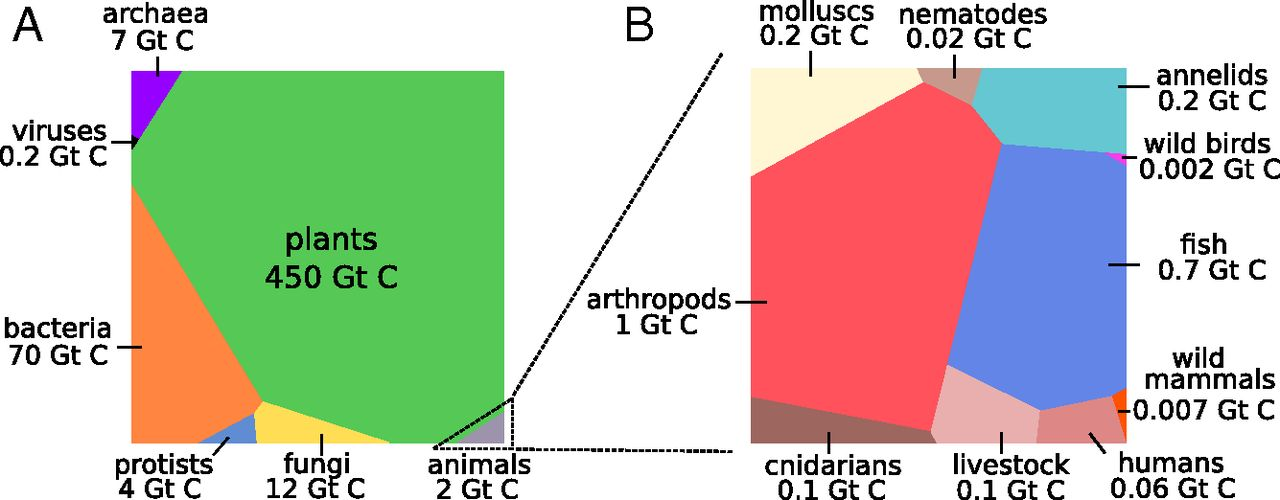
\includegraphics[width=0.7\linewidth]{static/biomass}
    \caption{
    \es{Distribución de la biomasa en el planeta tierra. }%
    }
    \label{fig:biomass}
\end{figure}
En el gráfico de la izquierda podemos ver que la plantas y las bacterias representan el 95\% de la biomasa de la tierra.
En este sentido, la capacidad de adaptación de la información que estas especies almacenan en su sistema genético es varios órdenes de magnitud superior al alcanzado por los seres humanos mediante sus complejos sistemas de información cultural.

\section{Cultura}

La especial integraci\'on de los procesos biol\'ogicos, cognitivos y sociales que permiten a los humanos desarrollar culturas complejas se debió a una coevolución genético-cultural que se desencadenó por el desarrollo previo de la crianza cooperativa~\cite{hrdy2020-emotionallyModern}.
Antes del surgimiento de los humanos \emph{anatómicamente} modernos (masa cerebral actual) y de los humanos \emph{conductualmente} modernos (lenguaje), surgió en África una linaje \emph{emocionalmente} moderno~\cite{hrdy2020-emotionallyModern}.
La forma en la que estos homininos organizaron la crianza produjo un ambiente que favoreció la selección de jóvenes capaces de monitorear y comprender las intenciones de los demás, y de atraer la atención de sus cuidadadores de modo de compartir sus propias necesidades.

% Parrafo

La empatía fue la que permitió el desarrollo del Homo sapiens: la comprensión mutua, la imitación, el lenguaje y finalmente la cultura.
Esta costosa habilidad cognitiva es especialmente eficiente para la adquisición de tradiciones complejas.
Lo que antes debía ser redescubierto una y otra vez mediante costosa experiencia individual, ahora podía ser transmitido a la siguiente generación.
La capacidad de adquirir comportamientos basados en la experiencia de otros sin tener que re-construirlos cada vez por prueba y error conduce un proceso de evolución y acumulativa cultural que permite a las poblaciones humanas adaptarse rápidamente ante cambios bruscos en el ambiente o migraciones a nuevos entornos.

% Parrafo

El surgimiento de la cultura produjo cambios radicales para nuestra especie.
Antes de la transición cultural, estuvimos en grave peligro de extinción, lo que se evidencia en la baja diversidad del genoma humano.
Luego de la transición cultural, en pocos años nuestra especie ocupó todos los nichos ecológicos de la tierra como ningún otro vertebrado terrestre lo había logrado antes.
Esta proeza se logró mediante los sistemas culturales y tecnológico desarrollados por sociedades cazadores-recolectores.
Caminando salimos de África, ocupamos Asia, y de allí Oceanía y las Américas (las flechas del mapa~\ref{fig:agricultura}).
La información transgeneracional fue la que le permitió a estas sociedades simples adaptarse rápidamente a los nuevos desafíos ecológicos.

% Parrafo

El cambio climático ocurrido al inicio del Holoceno (hace 12000 años) propició el desarrollo de la agricultura, que surgió de manera indendiente en los seis grandes sistemas geográficos de la tierra: en la región central de África subsahariana, en Asia occidental, en Asia oriental, en Oceanía norte, en América del norte y en América del sur (las puntos rojos del mapa~\ref{fig:agricultura}).
\begin{figure}[ht!]
    \centering
    \begin{subfigure}[b]{0.6\textwidth}
     \includegraphics[width=\textwidth]{figures/agricultura.pdf}
     \caption{Poblamiento de la tierra y agricultura}
     \label{fig:agricultura}
    \end{subfigure}
%     \begin{subfigure}[b]{0.40\textwidth}
%     \includegraphics[width=\textwidth]{static/polynesia.png} 
%     \caption{Poblamiento del océano Pacífico}
%     \label{fig:polynesia}
%     \end{subfigure}
    \caption{
    El mapa de la figura~\ref{fig:agricultura} es una proyección políedrica de la tierra que conserva los tamaños relativos de los continentes.
    Las felchas indican el poblamiento, desde África a Asia, y de Asia hacia Oceanía y América.
    Los puntos rojos indican surgimiento independiente de agricultura.
    El mapa de la figura~\ref{fig:polynesia}, desarrollado por Thorsby~\cite{thorsby2016-polynesiaAmerica}, muestra el poblamiento de la Polynesia y los contactos con Ámerica evidenciados en el material genéticos. }%
    \label{fig:poblamiento}
\end{figure}
Alrededor de estos puntos se desarrollaron los principales centros poblacionales de la humanidad.
El aumento de la población promovió, a su vez, el desarrollo de nuevas innovaciones tecnológicas y científicas, como la escritura, la matem\'aticas, las ingenier\'ias, la astronomía, las ciencias políticas, entre otras.
Durante el año 1400 el mundo florecía de sociedades "prósperas"~\cite{dussel2004-sistemaMundo}: Aztecas en Ámerica del norte, Incas en Ámerica del sur, Tongas en el Pacífico, Bantúes en África sub-sahariana, los Árabes e Indios en Asia occidental y Chinos en Asia oriental, por mencionar algunos.

% Parrafo

El desarrollo tecnológico de todas estas sociedades fue extraordinario. 
El imperio de Tonga ocupaba hace siglos todo el oc\'eano Pac\'ifico (figura~\ref{fig:polynesia}) con sorprendentes tecnologías de navegación que le habían permitido tener intercambios con América, que se evidencian en el componente genético de los pueblos de la Polynesia~\cite{thorsby2016-polynesiaAmerica, ioannidis2020-polynesiaAmerica}.
En la región Inca se había desarrollado un sistema de intercambios basado en la reciprocidad de trabajo (minka, ayni y mita) que le permitía a las comunidades administrar eficientemente el uso de los bienes comunes y al Estado desarrollar la infrastructura en el vasto territorio montañoso~\cite{murra}.
En la región Azteca se había desarrollado un extenso mercado regional con ciudades de hasta 300.000 habitantes, tres veces la ciudad de Venecia en esa misma época~\cite{www7.uc.cl}. %http://www7.uc.cl/sw_educ/historia/conquista/parte1/html/h54.html
El mundo \'Arabe comerciaba productos desde el Océano Pacífico, en las Filipinas, hasta el Oc\'eano Atl\'antico, en Marruecos, conectando las innovaciones culturales de distintos hemisferios del planeta~\cite{dussel}.
África siempre fue el continente más diverso cultural y genéticamente, pero quizás el centro más innovador en términos científicos y tecnologías haya sido la región de China~\cite{needham2004-generalConclusionsAndReflections}.

% Parrafo

La supervivenvia de las comunidades depende de la capacidad permanente de renovación de los vínculos interpersonales, de mantener la salud de su tejido comunitario que se requiere para toda buena coordinación cooperativa.
La experiencia acumulada a través de las generaciones por las más diversas comunidades del mundo condujo, de forma independiente, al desarrollo de tecnologías de sociabilidad sorprendentemente similares entre sí.
En todas ellas se pueden reconocer al menos dos mecanismos que cumplen la función de re-ciclar los v\'inculos interprersonales: los ritos festivos y los ritos coercitivos~\cite{segato2016-guerraContraLasMujeres}.
La misma naturaleza multiplicativa de los procesos evolutivos que había ofrecido una ventaja física para la agregación cooperativa de las formas de vida, favoreció también la aparición de instituciones culturales basadas en la reciprocidad.

% Parrafo

Uno de los desafíos más grandes que enfrenta toda comunidad para su superviencia es la administración exitosa de los sistemas ecológicos sobre los que se sostiene la alimentación de sus miembros.
Los sistemas vivos explotados mediante riego, pezca, recolección o caza, se los conoce como ``recursos de uso común''.
En ellos el óptimo se alcanza cuando todos los miembros cooperan, pero la estructura de pagos individuales incentiva la sobreexplotación del recurso, por lo que existe un único equilibrio en el que a todos individualmente les conviene no cooperar.
El juego más conocido y quizás el más sencillo que ejemplifica la matriz de pagos de los bienes comunes es el llamado dilema del prisionero.

% Parrafo

Imagina dos jugadores, cada uno de los cuales tiene que decidir (ignorando la decisión del otro jugador) si cooperar $C$ con otra persona o desertar $D$.
Cooperar tiene un costo $c$, para que la otra peronsa reciba un beneficio $b$, con $b > c$.
Desertar significa evitar el costo $c$ que implica entregar el beneficio $b$ a la otra persona.
Esto da como resultado la siguiente matriz de pagos.
\begin{equation}
    \bordermatrix{ & C & D \cr
      C & b-c & -c \cr
      D & b & 0  } 
\end{equation}
Obsérvese que a las personas les conviene cooperar mutuamente antes que desertar mutuamente, ya que $b - c > 0$.
Sin embargo, no importa la situación uno siempre está mejor sin cooperar: si la otra persona deserta, es mejor desertar que cooperar, ya que $0 > -c$; si la otra persona coopera sigue siendo mejor desertar que cooperar, ya que $b > b - c$.
De ahí el dilema: aunque la cooperación mutua es un resultado preferible que la deserción mutua, ningún jugador tiene el incentivo de cooperar.

% Parrafo

Para ilustrar el problema en términos de evolución cultural, imaginemos qué pasa si los comportamientos se imitan en la sociedad en función de su beneficio individual.
Supongamos una población compuesta enteramente por desertores.
Un comportamiento cooperador es incapaz de viralizarse debido a que cada vez que se encuentra con desertores pierde $-c$, mientras que los desertores nunca pierden, y al encontrarse con el cooperador incluso ganan $b$.
Así en la etapa de imitación, los desertores tendrán más éxito y el único cooperador será eliminado de la población de desertores.
Por el contrario, si la población está compuesta enteramente por cooperadores, la eventual aparición de un comportamiento desertor es capaz de viralizarse rápidamente por la diferenca de pagos que recibe cada estrategia.

% Parrafo

Desertar es la única estrategia evolutivamente estable en el dilema del prisionero, tal como lo hemos planteado.
¿Cómo es posible entonces la evolución de la cooperación?
La principal familia de solución consiste en darle estructura a la red de interacciones, de modo que los cooperadores interactúen con aquellos que también cooperan.
En biología, la relación estrecha entre parientes favorece los genes cooperadores en tanto que su descendencia probablemente también sea cooperadora.
La cooperación humana es única en el sentido de que tiene lugar en comunidades de un gran número de individuos relativamente no relacionados entre sí.
La reciprocidad directa ha sido el principal mecanismo observado en todas las sociedades del mundo: dar ayuda genera comúnmente una respuesta semejante a cambio~\cite{donMauss}.

% Parrafo

Imaginemos el dilema del prisionero \emph{iterado}, en el que con probabilidad $w$, se juega otra ronda, y que con probabilidad $1 - w$ el juego termina.
En este escenario existe una estrategia de reciprocidad directa, conocida como tit-for-tat (TFT), que es capaz de resisitir la aparición de desertores incodiconales (ALLD), que desertan en todas las rondas.
La estrategia TFT comienza cooperando en la primera jugada y luego responde con el mismo comportamiento previo de la otra persona, premiando la cooperación con cooperación y castigando la deserción con la deserción.
Cuando dos TFT juegan entre sí, ambos cooperan siempre y obtienen una recompensa esperada de $(b - c)/(1 - w)$ cada uno.
Cuando un TFT se encuentra a un ALLD, en la primera ronda pierde $-c$ para favorecer a su oponente con $b$, a partir de la cual ambos desertan hasta terminar la serie de iteraciones.
Dos ALLD siempre desertan y obtienen siempre $0$.
\begin{equation}
    \bordermatrix{ & TFT & ALLD \cr
      TFT & \frac{b-c}{1-w} & -c \cr
      ALLD & b & 0  } 
\end{equation}
La estrategia TFT es una evolutivamente estable siempre que $(b - c)/(1 - w) > b$ o, lo que es lo mismo $b/c > 1/w$, si la relación entre las personas es lo suficientemente estable en el tiempo.
La identidad comunitaria juega en este sentido un papel fundamental.
Lo que identifica a los sujetos colectivos, los pueblos, es la autopercepción por parte de sus miembros de compartir una historia común, que viene de un pasado y se dirige a un futuro, en el que los vínculos se mentienen aun a través de situaciones de disenso interno y conflictividad~\cite{segato2016-guerraContraLasMujeres}.

% Parrafo 

Los ritos coercitivos, presentes en todas las sociedades, no son otra cosa que ceremonias para la reactivación de flujos de intercambios rotos previamente por conflictos entre partes.
Están orientados el restablecimiento de los vínculos mediante los mecanismos de ``reparación'', ``conciliación'' y ``ayuda'' \cite{zaffaroni2013-cuestionCriminal}, haciendo uso de los tres tipos de intercambios posibles entre partes: 
($\rightarrow$) el acto en el cual el acusado (o sus representantes) da algo al acusante (o sus representantes);
($\leftrightarrow$) el acto en el cual el acusado y acusante (o sus representantes) dan y reciben mutuamente;
($\leftarrow$) el acto en el cual el acusado (o sus representantes) recibe algo del acusante (o sus representantes).
La expulsión del agresor de la comunidad sólo se prevee en casos extremadamente excepcionales, pues el primer derecho de sus miembros es el derecho a la comunidad \cite{segato}.

% Parrafo

La identidad comunitaria y los ritos corcitivos tienden a darle estabilidad a los vínculos interpersonales, lo que favorece la estabilidad evolutiva de los comportamientos reciprocitarios en porblaciones que ya son reciprocitarias.
Sin embargo, no resuelven el origen inicial de la reciprocidad, pues las estrategias reciprocitarias, como TFT, siguen siendo incapaces de viralizarse en poblaciones enteramente desertoras.
Aunque la reciprocidad no pueda viralizarse dentro de poblaciones enteramente desertoras, dado que $0>-c$, los grupos compuestos por comportamientos reciprocitarios pueden verse favorecidos respecto de los grupos compuestos por desertores.

% Parrafo

%Lo que sí queda claro, es que los grupos con comportamientos reciprocitarios funcionan mejor que los grupos 
%Si Para que esto ocurra parece necesario un mecanismo que favorezca unos grupos sobre otros.
Price

% Parrafo

Los estudios comparativos sobre instituciones exitosas en la administradores de bienes comunes concluyen que su capacidad de supervivencia a largo plazo está asociada con la presencia de las siguientes caracterísiticas:\vspace{-0.1cm}
\begin{description}\setlength\itemsep{-0.1cm}
 \item[1. Identidad comunitaria y territorial:] el reconocimiento de miembros y del sistema ecológico específico sobre el cual se ejerce la jurisdicción.
 \item[2. Normas acordes a la comunidad y el sistema ecológico:] Las normas son compatibles con las condiciones sociales y medioambientales locales.
 \item[3. Deliberación comunitaria:] La mayoría de los individuos involucrados en el sistema ecológico están autorizados a participar en la elaboración y modificación de sus normas.\setlength\itemsep{-0.1cm}
 \item[4. Conocimiento experto local:] La supervisión de los compartamientos de las personas el sistema ecológico está a cargo de los mismos miembros.\setlength\itemsep{-0.1cm}
 \item[5. Garantías de derechos comunitatrias:] Las sanciones son graduales, comienzan siendo muy bajas, y sólo raramente se decide la expulsión de la comunidad porque el primer derecho es formar parte de una comunidad.
 \item[6. Ritos festivos y coercitivos:] ceremonias de intercambio para el restablecimiento de los vínculos comunitarios mediante los mecanismos de ``reparación'', ``conciliación'' y ``ayuda''.
 \item[7. Autonomía comunitaria:] el reconocimiento de las comunidades vecinas a establecer sus propias normas.
 \item[8. Relaciones intercomunitarias] cuando un recurso de uso común está conectado a un sistema socioecológico más amplio, las actividades se organizan en múltiples capas anidadas.
\end{description}

% Parrafo

\todo[inline]{Ejemplo Bali, perfecto order}

% 

A pesar de todos los avances científicos, la ciencia metropolitana moderna no fue capaz de compensar la perdida de los conocimientos milenarios acumulados por las comunidades autónomas locales.
Los estudios comparados indican que las únicas instituciones capaces de administrar a largo plazo los bienes comunes, nunca fueron ni estatales ni privadas, son de tipo comunitarias histórico arraigo local~\cite{ostrom2009,ostrom1990}.
La masiva pérdida de diversidad cultural trajo como consecuencia la masiva pérdida de biodiversidad actual, una crisis ecológica sin precedentes.
Los conocimientos milenarios y sus instituciones adaptadas ecológicamente se pierden definitivamente en unas pocas generaciones.
En un mundo de comunidades debilitadas, la pedagogía de la crueldad fedual-colonial-moderna logra introducir la cosmovisión individualista e instrumental de nuestro tiempo: la naturaleza como cosa, las personas como cosas.
%La intervención irracional de un grupo de humanos sobre el sistema ecológico, reservorio del principal conocimiento empírico para la vida, es la analogía más acabada de la imposición de la mentira sobre la verdad.

\section{Ciencia}

Gracias a estar ubicada en uno de los principales centros geográficos del planeta, China pudo emerger como el corazón del sistema de intercambios planetarios~\cite{pomeranz2000}.
Para el año 1400, China llevaba al menos 2000 de continuidad socio-pol\'itica, y 900 a\~nos de un estado meritocr\'atico en el cual sus miembros eran elegidos a trav\'es de concurso público (examen imperial).
Inventa el acero en el siglo segundo, el papel en el siglo sexto, la imprenta en el siglo octavo, el papel moneda en el noveno, la br\'ujula en el onceavo.
Desarrolla infraestructuras como el canal navegable \emph{Da Yunhe} de más de 1700 kilómetros para conectar la ciudad de Pekín con otras ciudades importantes, y la famosa muralla que en total superó los 20000km de longitud.
China ya era de hecho el principal proveedor comercial del resto del mundo.
No parecían necesitar nada más afuera de sus fronteras.
Es así como a pesar de que desarrolla la flota más grand de la historia, dirigidas por Zheng He (1405-1433), el Gobierno Chino decide cerrarse fronteras adentro dándolas por finalizadas por completo.

% Parrafo

Así como la integración favorece los proceso de innovación y acumulación cultural, el asilamiento induce pérdidas masivas de información cultural.
Un ejemplo de aislamiento total bien documentado ocurre con la separación de Tasmania del continente Australiano por la subida del nivel del mar ocurrida a comienzos del Holonceno.
La evidencia arqueológica y etnohistórica indica que desde el principio del Holoceno las sociedades de Tasmania perdieron gran parte de su cultura tecnológica.
La principal hipótesis sugiere que la reducción del tamaño efectivo de la población (\emph{effective population size}) fue la causa más importante de estas pérdidas culturales~\cite{henrich2004-demographyAndCulturalEvolution}.

\begin{figure}[ht!]     
  \centering 
  \begin{subfigure}[c]{0.45\textwidth}
    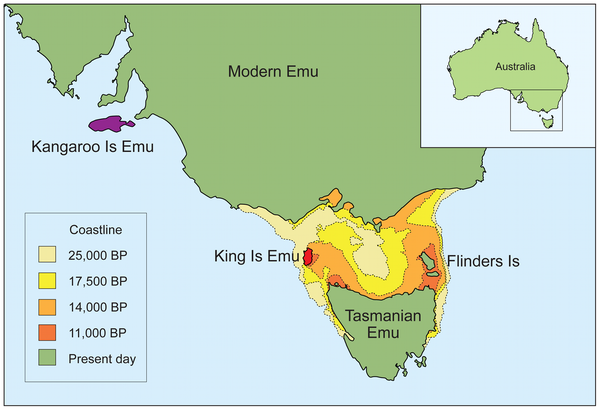
\includegraphics[width=\textwidth]{static/tasmania.png} 
    \caption{Tasmania}
    \label{fig:tasmania}
  \end{subfigure}
  \begin{subfigure}[c]{0.45\textwidth}
    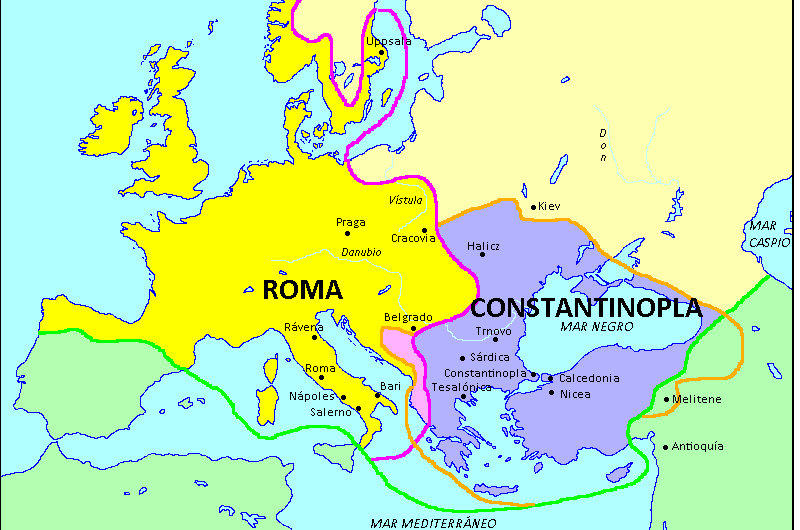
\includegraphics[width=\textwidth]{static/cisma.png} 
    \caption{Edad media}
    \label{fig:cisma}
  \end{subfigure}
  \caption{Aislamiento}
  \label{fig:aislamiento}
\end{figure}

Un caso de asilamiento parcial ocurre en Europa occidental.
Arrinconada ya en el lejano occidente por el fr\'io polar y la falta de tecnolog\'ias de navegaci\'on del Atlántico, Europa occidental comienza en el siglo octavo a quedar paulatinamente aislada del ``sistema mundo'' por la expansión Árabe al sur y por la serie cismas con el Imperio Bizantino al Oeste~\cite{Dussel}.
Esa etapa de aislamiento coincide con el proceso de perdida masivas de información cultural y de degradación de las condiciones socio-económicas conocido como ``edad media'', un proceso que sólo ocurre en Europa occidental.
Si no era posible recuperar el acceso al sistema mundo por el Oriente a través de las cruzadas, la única opci\'on que quedaba era explorar los mares del Este.

% Parrafo

Producto de la pésima situación socio-económica de la ``edad media'', apenas Europa occidental descubre cómo navegar el Atlántico, comienza un masivo proceso migratorio.
La coincidencia de un conjunto de eventos puso a esta sociedad, históricamente marginal, en una situación de privilegio mundial.
Un siglo antes, China hab\'ia incorporado la plata como monedad oficial, la que ya estaba siendo utilizada como moneda de cambio en todo el mundo Árabe~\cite{pomeranz2000-divergence, pomeranz2018-tradeCreated}.
En América del sur el estado incaico que estaba organizado en base a un sistema de intercamios no monetarios en una región montañosa rica en minerales precisosos.
Además de la buena predisposición con la que los exploradores reportan haber sido recibidos por los habitantes Americanos, la llegada de masiva de emigrantes feudales produjo una serie de pandemias que redujeron la población local en por lo menos 60\% entre los años 1500 y el 1600~\cite{koch2019-europeanArrival}.

% Parrafo

Cuando 1546 los exploradores descubren la montaña de plata de Potosí, en el centro del sistema estatal incaico, la Europa feudal queda inmediatamente en una posición de privilegio en todo el mundo afro-euro-asiático.
Mediante la captura del sistema administrativo incaico (golpe de estado) los impuestos que antes antes se destinaban al desarrollo de la infraestructura, comienza a ser utilizado para extraer la plata, un mineral sin interés por los nativos.
En poco tiempo la plata Árabe queda devaluada ante la inmensa cantidad de plata que llagaba de América.
Así es que 25 años después, en 1571, Europa occidental rompe en el Meditarraneo el asilamiento sufrido durante la edad media (batalla de Lepanto).
La integración privilegiada al sistema mundo inicia un proceso rápido de acumulación cultural basado en las tecnologías extranjeras.
La plata de América fluye en todas las direcciones, principalmente en dirección a China.

\begin{figure}[ht!]     
  \centering 
  \begin{subfigure}[b]{0.48\textwidth}
    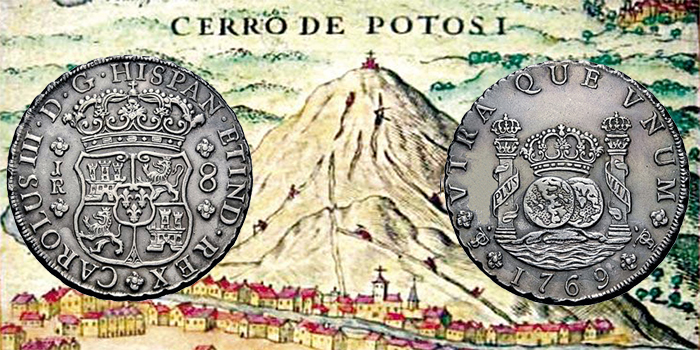
\includegraphics[width=\textwidth]{static/plata-potosi} 
    \caption{Plata}
    \label{fig:potosi}
  \end{subfigure}
   \ \ 
  \begin{subfigure}[b]{0.47\textwidth}
    \includegraphics[width=\textwidth]{figures/china.pdf} 
   \caption{Opio}
    \label{fig:china-pop}
  \end{subfigure}
  \caption{La plata y el opio como las llaves de la integración privilegiada de la Europa occidental en el sistema mundo.}
  \label{fig:integracion}
\end{figure}

Durante 250 años la plata americana sirvió para muchas cosas, pero principalmente para comprar productos chinos y financiar la primera industrialización británica con tecnología China.
Europa consumía productos asiáticos, pero exportaba muy poco a Asia.
El comercio internacional de opio comenzó en el 1700 como respuesta a una crisis del comercio internacional europeo, especialmente británico.
El opio, un producto lujoso utilizado en China como medicina (raramente como estupefaciente), fue prohibida por los emperadores chinos en 1729, que por su abundancia hacía crecer lentamente la cantidad de adictos.
Las consecuencias fueron más graves cuando en 1818 se desarrolla una mezcla de opio más barata y potente.

% Parrafo

Mediante el narcotráfico Europa occidental consigue por primera vez, en el siglo 19, revertir el déficit comercial que siempre tuvo con China, desde los tiempos del imperio romano.
El número de adictos llegó a ser lo suficientemente alarmante, y en 1839 China comete el error de declarar la guerra al narco-estado británico en su propio territorio.
Los resultados fueron terribles.
Los chinos no sólo no pudieron impedir el ingreso de la droga, perdieron también su autonomía arancelaria, el derecho a someter a los residentes extranjeros a la ley china.
Expuesta a su debilidad militar, China sufrió un siglo calamitoso de agresiones extranjeras, desorden interno y guerra civil, que produjo una caída de 1/5 de su población (figura~\ref{fig:china-pop}).

% Parrafo

Luego de la derrota de China por parte del narco-estado británico, se establece finalmente la hegemonía de Europa occidenta en el sistema mundo y se profundiza el proceso de colonización en todo el mundo. % que hasta el momento estaba limitado estatales de América continental estaba limitada a puertos e islas.
En 1850 comienza la colonización de África continental y de los extensos territorios americanos que todavía seguían a manos de comunidades locales.
Comienza la era de los genocidios.
Todos los conocimientos que la sociedad colonial va incorporando del resto de comunidades del mundo se les borra su verdadero origen histórico y se las enaltecen como surgimientos espontaneos internos.
Es una nueva era de avances científicos y tecnológicos, pero por otro es la era de pérdida de diversidad cultural.
En todas las partes del globo, los exploradores y etnógrafos fueron documentando la perdida de cultural debida al avance del frente colonial-moderno, estatal o privado, sobre las autonomías locales.

\begin{figure}[ht!]
    \centering
    \begin{subfigure}[b]{0.48\textwidth}
    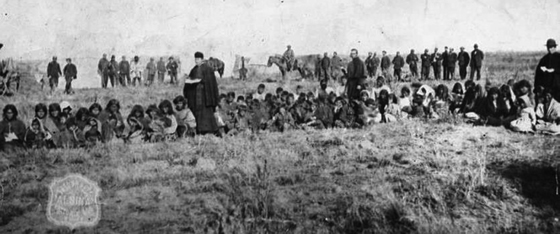
\includegraphics[width=\linewidth]{static/genocidio_patagonia}
    \caption{Genoetnocidios}
    \label{fig:genocidio_patagonia}
    \end{subfigure}
    \begin{subfigure}[b]{0.47\textwidth}
    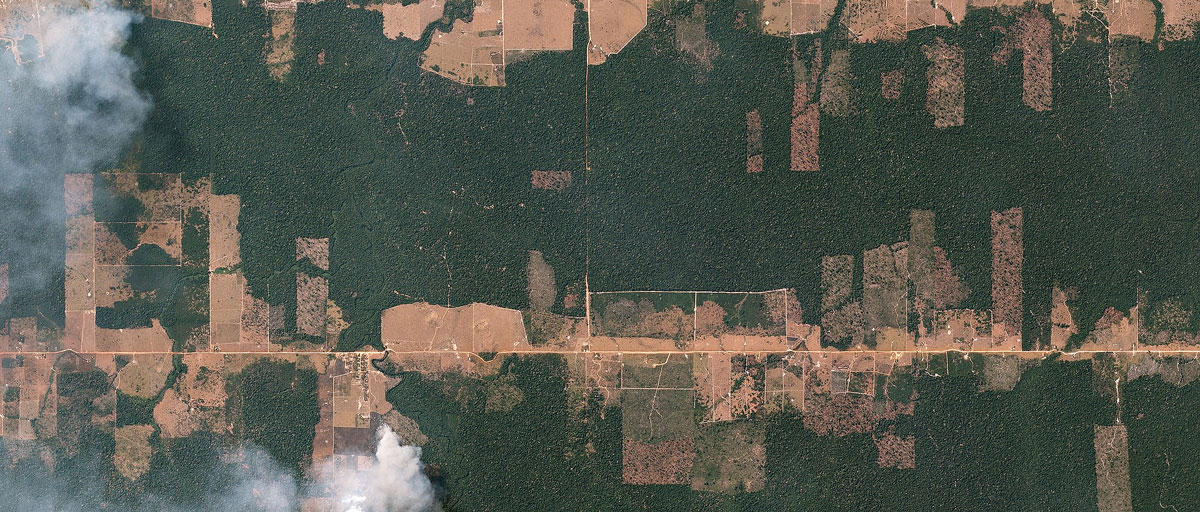
\includegraphics[width=\linewidth]{static/deforestation-brazil}
    \caption{Crisis ecológica}
    \label{fig:deforestation-brazil}
    \end{subfigure}
    \caption{
    La masiva pérdida de diversidad cultural trajo como consecuencia la masiva pérdida de biodiversidad actual, una crisis ecológica sin precedentes.
    }
    \label{fig:cultural-lose}
\end{figure}

\todo[inline]{brake}

Europa occidental también estuvo constituida por este tipo de comunidades.
Si bien el imperio romano eliminó una parte importante de este paisaje cultural, no alcanzó a eliminarlo por completo.
Los ``bárbaros'' justamente eran comunidades autónomas establecidas en la parte norte de Europa occidental, que persistieron luego de la caída del imperio romano de occidente.
Pero la ``edad media'' fue una anomalía en la historia de la humanidad.
En la etapa de aislamiento comenzó a ganar terreno al interior de la sociedad feudal el criterio de autoridad (sexual, militar, académica, moral) como fundamento del ``saber auténtico''.
Las instituciones heredadas del imperio romano de occidente, en cabeza de la iglesia católica romana, comenzaron a competir con las comunidades indígenas locales y a producir una conjunto de novedosas tecnologías de colonización~\cite{zaffaroni2013-cuestionCriminal}. 

% Parrafo

Una de las primeras y más importante tecnologías de colonización que desarrolla la iglesia católica romana es la regulación de las relaciones comunitaria de reproducción de forma más detallada que la propiedad.
Esta acción proscribe el rol político que las mujeres desempeñan en la administración del espacio doméstico comunitario, interviniendo en el funcionamiento de sus tecnologías de sociabilidad.
Se debilita así el arraigo comunitario, facilitando la captación de población desertora para actividades militares.
\begin{figure}[ht!]
    \centering
    
\includegraphics[width=0.18\linewidth]{static/digesto1553.jpg}
    
\includegraphics[width=0.213\linewidth]{static/malleus.jpeg}
    \caption{El criterio de autoridad como fundamento del ``saber auténtico'' y la guerra contra las mujeres como tecnología de colonización. %La proscripción de las tecnología de sociabilidad comunitaria, acción política del espacio doméstico administrada principalmente por las mujeres, debilita el arraigo comunitario facilitando la capatación de población desertora para actividades militares.
    }
    \label{fig:malleus}
\end{figure}
El poder punitivo se fue extendiendo y un nuevo sistema penal re-nació de los llamados \emph{libris terribilis} del Digesto, antiguas leyes romanas recolectadas por encargo del emperador Justiniano de Constantinopla pero re-interpretadas en occidente de modo de liberar al poder punitivo de todo límite.
En esta etapa, el sujeto masculino se torna modelo de lo humano y de todo cuanto sea dotado de politicidad, interés general y valor universal, y el espacio de las mujeres se transforma en margen y resto de la política.
La guerra contra las mujeres se formaliza definitivamente con la publicación del \emph{Malleus maleficarum} en 1484, que es el segundo best seller de la modernidad después de la Biblia durante los siguientes 200 años.

% Parrafo

Sólo después de que la sociedad feudal adquiere una posición de privilegio en el sistema mundo, comienza al interior de esta sociedad, ahora colonial-moderna, un nuevo debate sobre las fuentes de validación del conocimiento.
En esta etapa el criterio de experiencia personal comenzó ganar terreno como fundamento del ``saber auténtico'' sobre los criterios de autoridad.
Algunos lo entendieron la experiencia como ``evidencia intelectual'' (racionalistas) y otros como ``evidencia sensible'' (empiristas), dos grupos de exigencias que se consideraron al principio incompatibles entre sí: el de universalidad y necesariedad por un lado, y el de fuente y acreditación empírica por otro.
Sin embargo, de ambos lados existió un consenso de que el nuevo criterio, que servía para democratizar el conocimiento al interior de la sociedad feudal, estaba reservado para uso exclusivo de sus miembros varones.

% Parrafo

El argumento de la superioridad moral, que es utilizado durante toda la modernidad hasta el presente, lo desarrolla por primera vez Ginés de Sepúlveda cuatro años después del descubrimiento de la plata de Potosí, en 1550.
\begin{quotation}
 Será siempre justo y conforme al derecho natural que tales gentes [bárbaras] se sometan al imperio de príncipes y naciones más cultas y humanas, para que por sus virtudes y la prudencia de sus leyes, depongan la barbarie y se reduzcan a vida más humana y al culto de la virtud [...] Y si rechazan tal imperio se les puede imponer por medio de las armas, y tal guerra será justa según el derecho natural lo declara [...] En suma: es justo, conveniente y conforme a la ley natural que los varones probos, inteligentes, virtuosos y humanos dominen sobre todos los que no tienen estas cualidades~\cite{GinesdeSepulveda1967p87}.
\end{quotation}
Esta idea no se ve afectada por el argumento que propone Kant, conocido como el imperativo categórico, de que la validez del conocimiento radica en el reconocimiento mututo,
\begin{quotation}
Obra de tal modo que la máxima de tu voluntad pueda valer siempre al mismo tiempo como principio de una legislación universal \cite{Kant2003:28}.
\end{quotation}
El criterio de autoridad feudal-colonial-moderno sin embargo continúa latente en el mismo Kant, quien no percibe una contradicción cuando unos parrafos más adelante él mismo considera que las razas americanas son incapaces de toda cultura y que las razas negras pueden ser educadas pero sólo como sirvientes y esclavos.
No hay contradicción porque el concepto de ``universalidad'' fedual-colonial-moderno nace limitado.
Mujeres, extranjeros, animales y sistemas ecológicos completos participan sólo como objetos de los varones-blancos, estos últimos únicos sujetos con valor universal.
La sociedad colonial-moderna, y su ciencia, repite la estructura verticalista y punitivista de la sociedad feudal, ahora con alcance global gracias a la plata Americana.


% Parrafo

Todos los conocimientos que la nueva sociedad colonial-moderna va incorporando de todos los rincones del mundo, se les borra su verdadero origen histórico y se las enaltecen como surgimientos espontaneos internos.
Recién en 1800 Hegel propone por primera vez una periodización histórica que coloca a Europa occidental, que había sido históricamente marginal del sistema mundo, como centro y fin de la Historia Universal: \emph{antigüedad} - \emph{edad media} - \emph{modernidad}~\cite{dussel2007}. 
El mito eurocéntrico proyecta a la Europa feudal en la cultura griega y judeo-cristiana (ambos fenómenos de origen oriental) con pretensión de explicación histórico-mundial: ``la historia universal va del Oriente al Occidente; Europa es el centro absoluto de la historia universal'' dice Hegel~\cite{hegel}.

% \begin{figure}[ht!]
%     \centering
%     \begin{subfigure}[b]{0.15\textwidth}
%     \centering
%     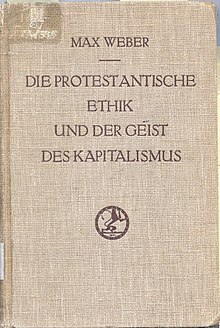
\includegraphics[width=\linewidth]{static/weber}
%     \caption{Weber}
%     \label{}
%     \end{subfigure}
%     \begin{subfigure}[b]{0.15\textwidth}
%     \centering
%     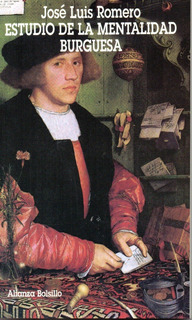
\includegraphics[width=0.9\linewidth]{static/romero}
%     \caption{Romero}
%     \label{}
%     \end{subfigure}
%     \begin{subfigure}[b]{0.15\textwidth}
%     \centering
%     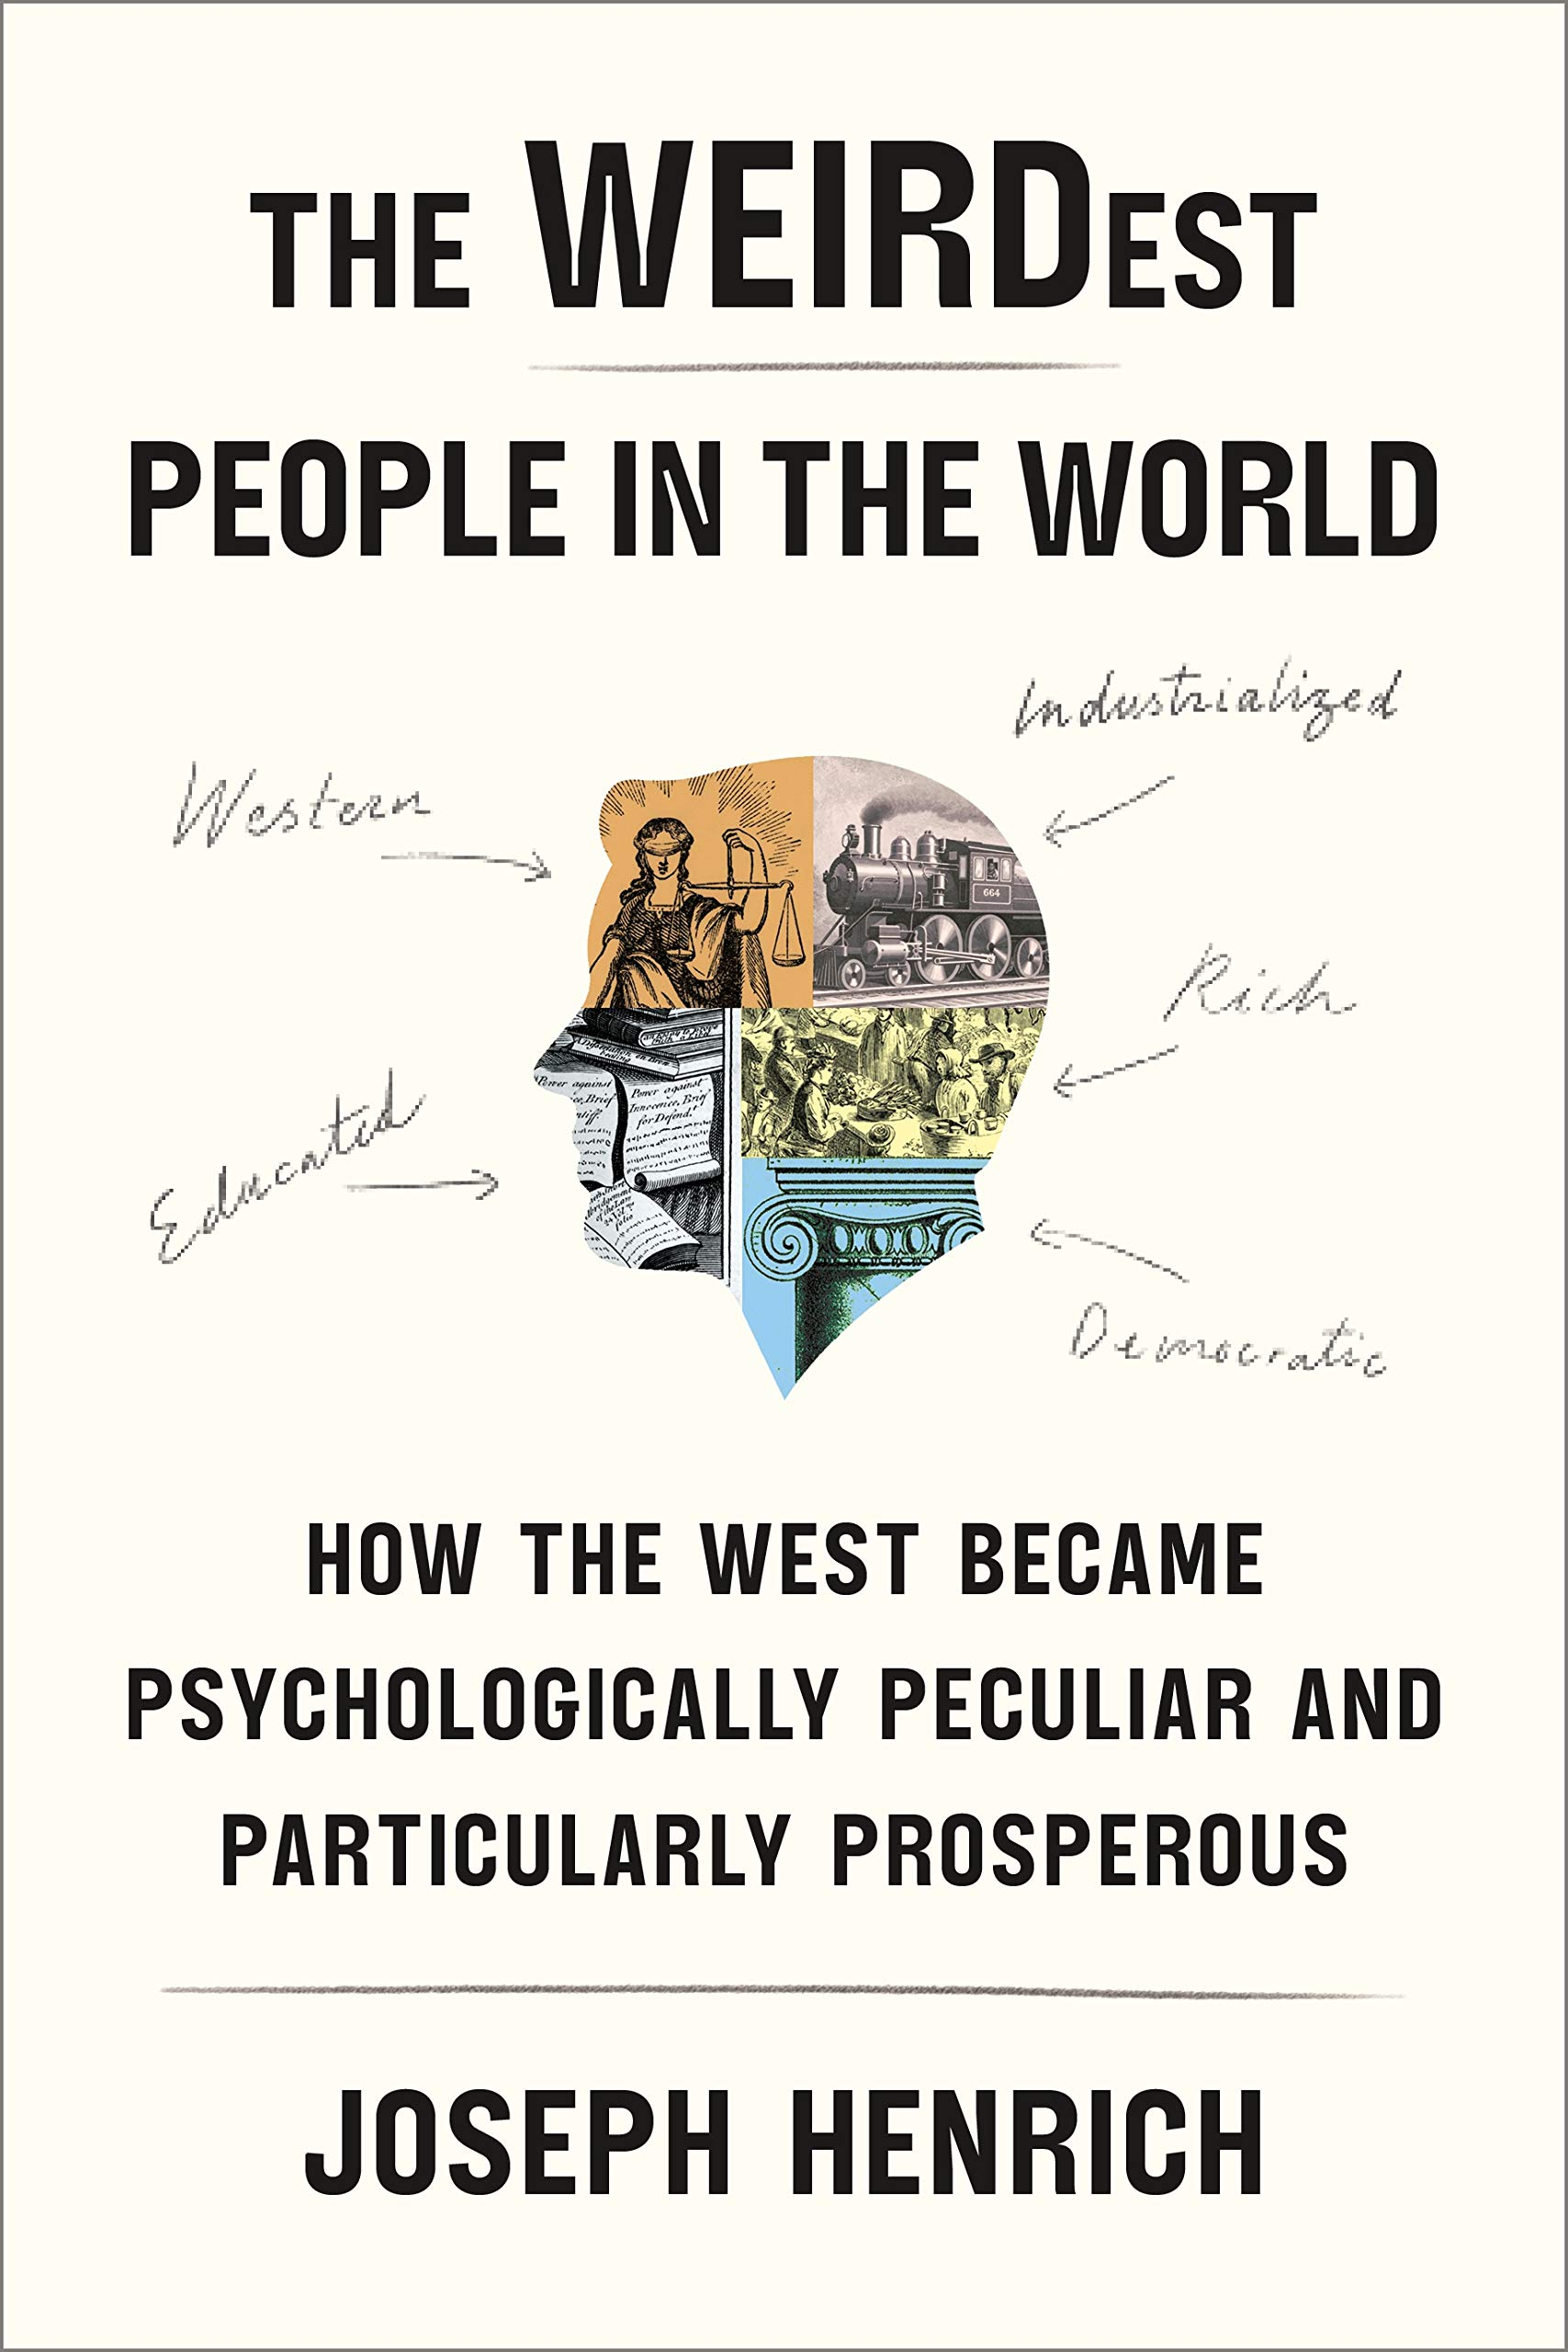
\includegraphics[width=1\linewidth]{static/henrich}
%     \caption{Henrich}
%     \label{}
%     \end{subfigure}
%     \caption{Mito eurocéntrico}
%     \label{fig:mito}
% \end{figure}

Este relato falso de la historia está vigente todavía hoy en la principales univerisidades del mundo occidental, desde Harvard a la Universidas de Buenos Aires, tanto en universidades de África, el mundo Árabe, India y Asia.
Desde Hegel hasta la fecha, las explicaciones eurocéntricas intentan explicar la proposperidad actual de occidente a través de una causa interna: el ``espíritu protestante'' de Weber \cite{weber}, la ``mentalidad burguesa'' de Romero \cite{romero}, o más recientemente el ``sistema de parentezco''\cite{henrich} de Henrich.
La paradoja que no puede responder el relato eurocéntricos es cómo una sociedad sumida en un proceso de involución cultural, como la sociedad feudal de la ``edad media'', pudo generar de repenten el proceso de desarrollo científico y técnico de la modernidad.

% Parrafo

Ninguna de las explicaciones eurocéntricas incorpora en su análisis la situación de aislamiento que sufre Europa occidental en la etapa previa ni la posterior situación de integración privilegiada en el sistema mundo.
Incluso Needham, el británico que recopiló la monumental historia científica y técnica de China, reconoce que comenzó a estudiar el tema motivado por responder la pregunta de por qué sólo Europa occidental había logrado el avance científico.
\begin{quotation}
When I first formed the idea, about 1938, (...) I regarded the essential problem as that of why modern science had not developed in Chinese civilisation (or Indian or Islamic) but only in that of Europe~\cite{needham2004-generalConclusionsAndReflections}.%
\end{quotation}
Luego de 60 años de investigaciones, Needham se ve obligado inviertir la pregunta.
\begin{quotation}
Why, between the -1th century and the 15th century, was Chinese civilisation much \emph{more} efficient than occidental in gaining natural knowledge and in applying it to practical human needs?~\cite{needham2004-generalConclusionsAndReflections}
\end{quotation}

% Parrafo

La Europa feudal no se había despertando del impacto de su invasión colonial cuando ya en 1514 Bartolomé de la Casas inicia desde América la advertencia de los efectos negativos de la integración basada en la dominación que promovían los primeros migrantes feudales.
En su crítica Bartolomé:
a) refuta la pretensión de superioridad de la cultura occidental sobre las las culturas indígenas;
b) diferencia entre otorgar al otro (al indio) pretensión universal de verdad, sin renunciar a la pretensión de predicar a favor la propia cultura cristiana;
c) y demuestra la falsedad del argumento usado para justificar la intervención en las autonomías locales, basado en el supuesto ``remedio a las injusticias internas'', en tanto esa intervenciones producían peores efectos sobre las poblaciones intervenidas.

% Parrafo

El criterio de autoridad globalizado durante la colonial-modernidad como criterio de universalidad limitado a los varones blancos abrió la puerta a la aribitrariedad cultural y ecológica.
En efecto, luego de cinco siglos podemos ratificar sus efecto negativos: la masiva perdida de diversidad cultural primero y la masiva pérdida de biodiversidad en curso en la actualidad.
La completa universalización del imperativo de convivencia no se sustenta en argumentos relativistas, que reclaman el derecho de los pueblos a la mera diversidad cultural.
El derecho a las autonomías comunitarias se sustenta en el hecho práctico de que el único conocimiento cultural ecológicamente adaptado evoluciona sólo a través de la experiencia que acumulan los pueblos en el transcurso de su historia~\cite{Rita}.

\begin{figure}[ht!]
    \centering
    \begin{subfigure}[b]{0.45\textwidth}
    \centering
    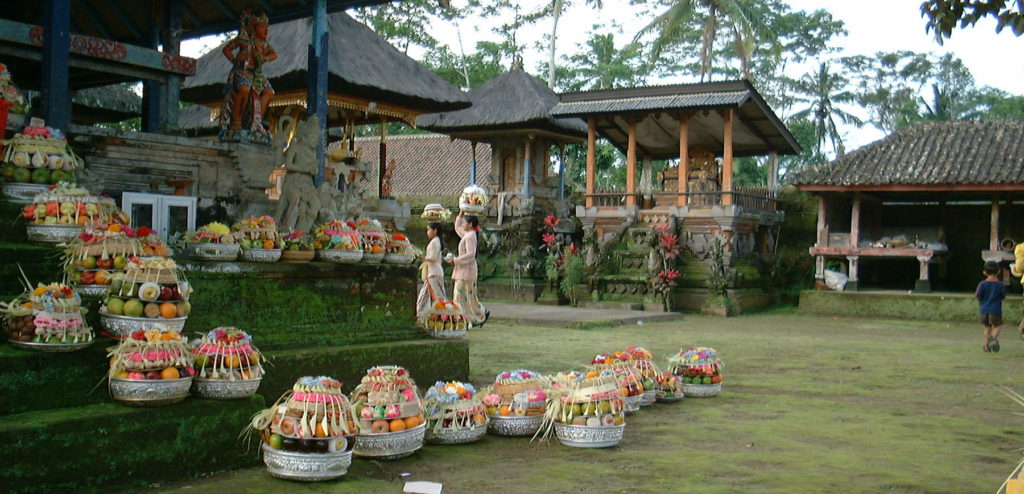
\includegraphics[width=\linewidth]{static/bali-offerings}
    \caption{Canang sari}
    \label{}
    \end{subfigure}
    \begin{subfigure}[b]{0.33\textwidth}
    \centering
    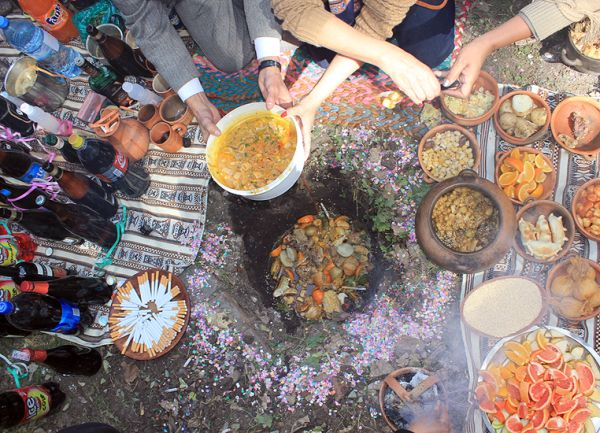
\includegraphics[width=\linewidth]{static/pachamama}
    \caption{Pachamama}
    \label{}
    \end{subfigure}
    \caption{La Madre Naturaleza como sujeto de derecho.}
    \label{fig:mito}
\end{figure}

El reconocmiento mutuo, que estuvo en la base de la evolución de nuestra especie, debe adquirir una universalidad que ni la propuesta parcial de Kant ni la cultura colonial-moderna ha sido capaz de alcanzar.
Es necesario que el imperativo de convivencia ``Obra de tal modo que la máxima de nuestra voluntad pueda valer siempre al mismo tiempo como principio de una legislación universal'' sea efectivo, reconociendo esta vez como sujetos con valor universal: al estatus social y político que las mujeres encabezan en el espacio comunitario; las autonomías comunitarias; y los derechos de las otras especies y de la madre tierra toda (\emph{pachamama}) de no ver interrumpido sus procesos ecológicos sin justa causa: lo mínimo necesario para el buen vivir (\emph{suma kausay}).

\section{Funciones}

El criterio de universalidad, como fuente de validez del conocimiento, nos obliga a rechazar la superiordad moral de subjetividades especiales de grupos particulares.
Este principio de convivencia, basado en el reconocimiento mutuo, reconoce ya que el conocimiento válido es quel que se alcanza a través de una actividad constructiva entre sujetos y no como la imposición automática del objeto al sujeto (objetividad), pues son los sujetos quienes activamente buscan el equilibrio de sus subjetividades sobre los objetos (acuerdos intersubjetivos).
Para el proyecto intercultural de acuerdos intersubjetivos, que se propone la ciencia, se hace necesario contar con herramientas que permitan a los individuos poner en correspondencia unívoca los fenómenos percibidos por sus conciencias individuales con algún esquema de operación que sea públicamente inteligible y reproducible.
En este sentido, las funciones ocupan un rol fundamental.

% parrafo

En su definición formal, una función es una relación (u operación) $f$ que a cada elemento de un conjunto (dominio) $X$ asigna un único elemento de otro conjunto (imagen) $Y$.
%
\begin{equation}
 \forall x \in X \  \exists! y \in Y \text{ tal que } f(x) = y    
\end{equation}
%
A primera vista puede parecer que las funciones no tienen nada en especial respecto de otro tipo de relaciones posibles entre conjuntos.
Sin embargo, lo que hace tan poderosa a las funciones como herramienta para la ciencia es el hecho de que ellas permiten definir asignaciones no ambiguas.

% Parrafo

Los funciones son la base de las ciencias formales.
Todos los sistemas matemáticos de interés están compuestos por axiomas $X$, una serie de operaciones válidas $F$, y un conjunto de consecuencias $Y$ consistentes entre sí.
En teoría de la computabilidad, la tesis de Church-Turing afirma que toda función sobre los números naturales puede ser calculada por un ``método efectivo'' si y sólo si es computable por una máquina de Turing.
Debido a que todos las definiciones alternativas del concepto  de ``método efectivo'' resultaron ser equivalentes a una maquina de Turing, actualmente se supone que la hipótesis Church-Turing es cierta.

% Parrafo

Las funciones son también la base de las ciecias empíricas.
Veremos cómo los tres conceptos fundamentales de toda teoría empírica, los modelos causales, los datos y la incertidumbre tienen una estructura funcional.
Al final de esta sección introduciremos el concepto funcional de honestidad como método general para la validar el conocimiento empírico.

\subsection{Modelos causales}

La tendencia por entender la naturaleza en términos de mecanismos ocultos de causa y efecto, está extendida en todas las culturas.
Este idea de que todo lo que ocurre debe tener una causa previa que lo genere se conoce en la historia de la filosofía como el pricipio de \emph{razón suficiente}.
El concepto de causa y efecto tiene nuevamete una estructura funcional, $f(x) = y$, donde $x$ representa las condiciones iniciales, $f$ el modelo causal determinista, e $y$ el efecto.
Sin presencia de factores aleatorios, las condiciones iniciales generan siempre el mismo destino inevitable.
Esta idea llevada al extremo, la de un mundo totalmente determinista, es rechazada tanto por experimentos de la física cuántica como por el supuesto teórico sobre el libre albedrío de las ciencias sociales.
Sin embrago, los modelos causales deterministas se usan cotidianamente en todas las ramas de la ciencias empíricas para representar el funcionamiento del mundo.

% Parrafo

Por ejemplo, consideremos por un minuto el problema de conocer c\'omo cambian las habilidades individuales a lo largo del tiempo, tema sobre el que nos enfocaremos en el transcurso de esta tesis.
Dado que la habilidad es muchas veces una variable ocultas, lo mejor que podemos hacer en esos casos es estimarlas a partir de sus consecuencias observables directas: el producto de la resoluci\'on de problemas y competencias.
Rápidamente se percibió que considerar s\'olo la frecuencia de resultados positivos como indicador de la habilidad de los individuos conduce generalmente a aproximaciones erroneas, fundamentalmente porque su valor depende tambi\'en de la dificultad de los desaf\'ios.
Por esta raz\'on, todos los estimadores de habilidad ampliamente usados se basan en comparaciones por pares.

% Parrafo

\begin{figure}[ht!]     
 \centering
  \tikz{         
    \node[det] (r) {$r$} ; 
    \node[const, left=of r, xshift=-2.35cm] (r_name) {\small \en{Result}\es{Ganar/perder}:}; 
    \node[const, right=of r] (dr) {\normalsize $ r = (d>0)$}; 

    \node[latent, above=of r, yshift=-0.45cm] (d) {$d$} ; %
    \node[const, right=of d] (dd) {\normalsize $ d=p_i-p_j$}; 
    \node[const, left=of d, xshift=-2.35cm] (s_name) {\small \en{Difference}\es{Diferencia}:};
    
    \node[latent, above=of d, xshift=-0.8cm, yshift=-0.45cm] (p1) {$p_i$} ; %
    \node[latent, above=of d, xshift=0.8cm, yshift=-0.45cm] (p2) {$p_j$} ; %
    \node[const, left=of p1, xshift=-1.55cm] (p_name) {\small \en{Performance}\es{Desempeño}:}; 

    \node[latent, above=of p1,yshift=0.7cm,fill=white] (s1) {$s_i$} ; %
    \node[latent, above=of p2,yshift=0.7cm,fill=white] (s2) {$s_j$} ; %
    
    \node[latent, above=of p1,xshift=-1cm, yshift=-0.45cm,fill=white] (u1) {$u_i$} ; 
    \node[latent, above=of p2,xshift=1cm, yshift=-0.45cm,fill=white] (u2) {$u_j$} ; 
    \node[const, left=of u1, xshift=-0.55cm] (u_name) {\small \en{Others factors}\es{Otros factores}:}; 
    
    \node[const, right=of p2] (dp2) {\normalsize $p = s + u$};

    \node[const, left=of s1, xshift=-1.55cm] (s_name) {\small \en{Skill}\es{Habilidad}:}; 
    
    \edge {d} {r};
    \edge {p1,p2} {d};
    \edge {s1} {p1};
    \edge {s2} {p2};
    \edge {u1} {p1};
    \edge {u2} {p2};
  }
  \caption{Modelos causal determinista en el que las habilidades y otros factores causan los resultados observables a través de la diferencia de rendimientos, $d=p_i-p_j$: quien haya obtenido mayor rendimiento gana, $r = (d > 0)$.
  Las flechas representan relaciones causales.
  Los círculos representan variables continuas, y los cuadrados variables discretas.}
  \label{fig:elo_deterministas}
\end{figure}

% Parrafo

Desde los primeros modelos, propuestos hace casi un siglo por~\cite{Thurstone1927} y~\cite{Zermelo1929}, se supone un resultado observado $r$ (ganar/perder) depende de la habilidad $s$ del los agentes y de otros factores $u$ (Figura~\ref{fig:elo_deterministas}).
Si el modelo fuera cierto y conociéramos con precisión tanto el valor de habilidad y de los otros factores involucrados durante cada partida, sabríamos con certeza quién ganaría en cada caso.
La variedad de comportamiento que puede adquirir este modelo es bastante reducida.
Sin embargo, modelos deterministras aun más simples pueden desarrollar comportamientos de una complejidad tal que se hacen impredecibles.

% Parrafo

Un ejemplo de sistema determinista capaz de adquirir comportamientos imprevisibles es el siguiente modelo ``poblacional''.
El modelo establece que el tamaño de una población, medida como proporción respecto de la capacidad máxima de un sistema, depende exclusivamente de su tamaño en el tiempo anterior y de un factor de reproducción $r$.
\begin{equation}
 \text{Población}(t+1) = r \cdot \text{Población}(t)\cdot (1-\text{Población}(t))
\end{equation}
Dependiendo del factor de reproducción y de la población inicial, vamos diferentes tipos de comportamiento.
En la figura~\ref{fig:poblacion} podemos ver tres comportamientos típicos.
\begin{figure}[ht!]
    \centering
    \begin{subfigure}[b]{0.32\textwidth}
    \includegraphics[page=3,width=\linewidth]{figures/poblacion.pdf}
    \caption{Punto fijo}
    \label{fig:poblacion_punto_fijo}
    \end{subfigure}
    \begin{subfigure}[b]{0.32\textwidth}
    \includegraphics[page=9,width=\linewidth]{figures/poblacion.pdf}
    \caption{Periódico}
    \label{fig:poblacion_periodico}
    \end{subfigure}
    \begin{subfigure}[b]{0.32\textwidth}
    \includegraphics[page=11,width=\linewidth]{figures/poblacion.pdf}
    \caption{Caótico}
    \label{fig:poblacion_caotico}
    \end{subfigure}
    \caption{
    Tipos de atractores a medida que aumentamos el valor del reproducción $r$
    }
    \label{fig:poblacion}
\end{figure}
Cuando el valor del parámetro $r$ es chico (figura~\ref{fig:poblacion_punto_fijo}) la población tiende a un valor fijo, sin importar el tamaño inicial de la población.
Cuando el valor del parámetro $r$ es intermedio (figura~\ref{fig:poblacion_periodico}) la población oscila en un período.
Cuando el valor del parámetro $r$ llega a su límite (figura~\ref{fig:poblacion_caotico}) la población tiene un comportamiento denominado ``caótico''.

% En la figura~\ref{fig:camino_al_caos} graficos como va ocurriendo el cambio a medida que cambiamos el parámetro $r$.
% \begin{figure}[ht!]
%     \centering
%     \includegraphics[width=0.5\linewidth]{figures/camino_al_caos}
%     \caption{Los puntos a los que converge el sistema luego de 1000 iteraciones temporales.}
%     \label{fig:camino_al_caos}
% \end{figure}

Una de las propiedades más interesantes del atractor caótico es la sensibilidad a las condiciones inciales.
Si hacemos zoom en los primeros 30 pasos temporales de la figura~\ref{fig:poblacion_caotico}, y observamos el comportamiento del sistema al modificar levemente las condiciones iniciales, veremos que rápidamente las historias divergen completamente.
\begin{figure}[ht!]
    \centering
    \begin{subfigure}[b]{0.4\textwidth}
    \centering
    \includegraphics[page=13,width=\linewidth]{figures/poblacion}
    \caption{}
    \label{fig:sensibilidad}
    \end{subfigure}
    \begin{subfigure}[b]{0.4\textwidth}
    \centering
    \includegraphics[page=14,width=\linewidth]{figures/poblacion}
    \caption{}
    \label{fig:pseudo_aleatorio}
    \end{subfigure}
    \caption{(\subref{fig:sensibilidad}): Los primeros 30 puntos de la figura~\ref{fig:poblacion_caotico}. La linea negra comienza con una población de $0.5$ y la roja de $0.499$. (\subref{fig:pseudo_aleatorio}): Los primeros 2000 puntos de la figura~\ref{fig:poblacion_caotico}. La generación de números tiene un comportamiento pseudo aleatorio.}
    \label{fig:propiedades_caoticas}
\end{figure}
A pesar de que el modelo sea totalmente determinista, la sensibilidad a las condiciones iniciales impone un límite a la capacidad predicitiva.
Por más que la natrualeza sea determinista y conozcamos el mecanismo subyacente, si el sistema se encuentra en atractor caótico, jamás vamos a poder predecir el destino inevitable más allá de cierto tiempo debido a que en un sistema natural no podemos medir con infinita precisión las condiciones inciales.
La imposibilidad de determinar si estamos en presencia de las ``mismas condiciones iniciales'' es una fuente de incertidumbre que tiene toda ciencia empírica.

\subsection{Incertidumbre}

La teoría de la probabilidad es actualmente el enfoque más aceptado y utilizado para representar incertidumbre asociada al conocimiento empírico.
Las reglas de la probabilidad pueden derivarse formalmente a partir de una gran cantidad de sistemas axiomáticos conceptualmente distintos e independientes entre sí, lo cual es uno de los punto fuerte a su favor.
Ciertamentese ha dedicado mucho más esfuerzo a justificar la teoría de la probabilidad que cualquier otro enfoque para representar la incertidumbre y el tiempo dirá si se pueden se pueden desarrollar otros enfoques superadores.

% Parrafo

Es interesante cómo en contacto con problemas empíricos surgen, incluso en las ciencias matemáticas, diferentes escuelas de pensamiento.
La escuela frecuentista, tal como se enseña en la materia probabilidad y estadísitica de la facultad de ciencias exactas y naturales, define a la probabilidad como el número al que tiende una frecuencia obtenida luego de realizar varios ``experimentos independientes'' bajo ``las mismas condiciones''.
La probabilidad de eventos deterministas, según esta corriente, siempre es 0 o 1 aunque no conozcamos su valor.
Luego, la escuela frecuentista afirma que existen ciertas circunstancias en las dadas las mismas condiciones el sistema es capaz de evolucionar ``aleatoriamente'' en más de una dirección.
Estos objetos no deterministas que llaman ``variables aleatorias'' son el foco del interés de la corriente frecuentista.

% Parrafo

Sin embargo, hasta ahora no se ha encontrado ningún ``método efectivo'' que permita computar el comportamiento que se espera tenga una variable aleatoria.
Todas las soluciones sintéticas, desarrolladas exclusivamente con máquinas de Turing, son secuencias de números deterministas que tienen propiedades que se ``asemejan'' al comportamiento esperado de los variables aleatorias.
El modelo de poblaciones con $r = 3.99$ es un candidato interesante para simular números aleatorios.
En la figura~\ref{fig:pseudo_aleatorio} podemos ver que los primeros 2000 valores de esta función con una condición inicial $0.5$ parece tener una comportamiento aleatorio.
No son aleatorios justammente porque todos esos valores los podemos comprimir con la función y el valor de sus parámetros.
Nadie ha podido crear hasta ahora ``verdaderas'' variables aleatorios sin acudir al ruido natural.
%No podemos liberanos de las funciones a pesar de que queramos.

% Parrafo

A pesar de que no se haya encontrado un método sistemático para la generación de números aleatorios, las ciencias físicas y las ciencias sociales afirman que el mundo no tiene forma de función.
Por ejemplo, en las ciencias sociales el concepto de libre albedrío afirma que una persona expuesta ante un estado del universo tiene la capacidad de elegir una acción.
\begin{figure}[ht!]
\centering
    \scalebox{1}{
 \tikz{ %
        \node[estado] (s) {};
        \node[const, above=of s] {$s$};
        \node[accion, below=of s, xshift=-1cm] (a1) {} ; %
	\node[accion, below=of s, xshift=0cm] (a2) {} ; %
	\node[accion, below=of s, xshift=1cm] (a3) {} ; %
	\node[const, right=of a3] {$a$};
        \edge[-] {s} {a1,a2,a3};
      
	\node[estado, below=of a1,xshift=0cm] (s1a) {}; %
	  
	\node[estado, below=of a2,xshift=0cm] (s2a) {}; %
	   
	\node[estado, below=of a3,xshift=0cm] (s3a) {}; %
	    
	\node[const, right=of s3a] {$s^{\prime}$};
	\edge[-] {a1} {s1a};
	\edge[-] {a2} {s2a};
	\edge[-] {a3} {s3a};
        }
    
    }
    \caption{El concepto teórico libre albedrío afirma que una persona, ante un estados $s$ del universo, es capaz de elegir entre más de una acción $a_i$.}
    \label{fig:libre_albedrio}
\end{figure}
Sea porque el mundo natural admite la posibilidad de que un efecto surga sin su propia causa, o sea por nuestra incapacidad de reconocer el mundo en pleno detalle, situaciones como la descrita en la figura~\ref{fig:libre_albedrio} introducen incertidumbre.
Ya no es posible definir una función tal que dados los estados devuelva la acción, $f(s) = a_i$.

% Parrafo

La escuela bayesiana, a diferencia de la frecuentista, no afirma nada respecto de la naturaleza determinsta o aleatoria del mundo.
Cuando la incertidumbre nos impide conocer la función, podemos todavía expresar nuestra incertidumbre utilizando funciones de probabilidad, $P : \ \text{Acciones} \mapsto \mathbb{R}$.
Las funciones de probabilidad nos permiten inidicar nuestra ``distribución de creencias''.
En este caso supongamos que sabemos que las acciones sobre las que puede eligr la persona es dónde esconder un regalo.
¿Cómo podemos representar nuestra incertidumbre?
\begin{figure}[ht!]     
 \centering
 \tikz{
    \node[factor, minimum size=0.8cm] (p1) {} ;
    \node[factor, minimum size=0.8cm, xshift=1.5cm] (p2) {} ;
    \node[factor, minimum size=0.8cm, xshift=3cm] (p3) {} ;
    
    \node[const, above=of p1, yshift=.15cm] (fp1) {$P(a_1)$};
    \node[const, above=of p2, yshift=.15cm] (fp2) {$P(a_2)$};
    \node[const, above=of p3, yshift=.15cm] (fp3) {$P(a_1)$};
    } 
 \caption{Espacio de hipótesis: sabemos que hay un regalo detrás de sólo una de las tres cajas.}
 \label{fig:espacio_de_hipotesis}
\end{figure}
La figura~\ref{fig:espacio_de_hipotesis} nos ofrece suficiente información para definir un espacio de hipótesis: las tres cajas.
Sin embargo hay infinitas distribuciones de creencias posibles.
Por ejemplo, podemos tener el presentimiento de que está en la caja del medio.
En la figura \ref{fig:distribucion_de_creencias} mostramos dos posibles distribuciones de creencias que tienen preferencia esa caja.

\begin{figure}[ht!]     
 \centering
 \begin{subfigure}[b]{0.48\textwidth}
 \centering
  \tikz{ %
         \node[factor, minimum size=0.8cm] (p1) {} ;
         \node[factor, minimum size=0.8cm, xshift=1.5cm] (p2) {} ;
         \node[factor, minimum size=0.8cm, xshift=3cm] (p3) {} ;
         
         \node[const, above=of p1, yshift=.15cm] (fp1) {$0$};
         \node[const, above=of p2, yshift=.15cm] (fp2) {$1$};
         \node[const, above=of p3, yshift=.15cm] (fp3) {$0$};        
        }
    \caption{Preferencia total}
    \label{fig:preferencia_total}
 \end{subfigure}
 \begin{subfigure}[b]{0.48\textwidth}
 \centering
  \tikz{ %
         \node[factor, minimum size=0.8cm] (p1) {} ;
         \node[factor, minimum size=0.8cm, xshift=1.5cm] (p2) {} ;
         \node[factor, minimum size=0.8cm, xshift=3cm] (p3) {} ;
         
         \node[const, above=of p1, yshift=.15cm] (fp1) {$1/10$};
         \node[const, above=of p2, yshift=.15cm] (fp2) {$8/10$};
         \node[const, above=of p3, yshift=.15cm] (fp3) {$1/10$};        
        } 
    \caption{Preferencia parcial}
    \label{fig:preferencia_parcial}
 \end{subfigure}
\caption{Dos distribución de creencias que tienen preferencia por una de las hipótesis.}
 \label{fig:distribucion_de_creencias}
\end{figure}

La distribución de creencias de la figura~\ref{fig:preferencia_total} representa la certeza de que el regalo está en la caja del medio, mientras que la figura~\ref{fig:preferencia_parcial} representa una preferencia parcial que mantiene todavía cierta duda.
Pero si de verdad no tenemos ninguna información respecto de dónde está el regalo, ninguna de estas distribuciones parece ser una buena idea.
Más allá de los presentimientos personales de cada quién, podemos fácilmente llegar a un acuerdo respecto de que, dada la información disponible, no hay motivos para tener preferencia por ninguna de las opciones.
En este caso, una distribución de creencias honesta sería repartir la creencia en partes iguales, como mostramos en la figura~\ref{fig:distribucion_de_creencias_honesta}.

\begin{figure}[ht!]     
 \centering
\tikz{ %
        
         \node[factor, minimum size=.8cm] (p1) {} ;
         \node[factor, minimum size=.8cm, xshift=1.5cm] (p2) {} ;
         \node[factor, minimum size=.8cm, xshift=3cm] (p3) {} ;
         
         \node[const, above=of p1, yshift=.15cm] (fp1) {$1/3$};
         \node[const, above=of p2, yshift=.15cm] (fp2) {$1/3$};
         \node[const, above=of p3, yshift=.15cm] (fp3) {$1/3$};        
        } 
\caption{Distribución de creencias honesta cuando no tenemos información previa.}
 \label{fig:distribucion_de_creencias_honesta}
\end{figure}

Si llegamos a un acuerdo respecto de que no tenemos información previa, entonces estaremos de acuerdo en esta distribución de creencias.
Esta distribución de creencias, que permite el acuerdo intersubjetivo, la vamos a llamar creencia honesta.

% Parrafo

Es interesante notar que la creencia honesta, cuando no tenemos información previa, es la que maximiza la incertidumbre dividiendo la certidumbre en partes iguales.
Este se conoce como el \textbf{principio de indiferencia}.
En la sección~\ref{sec:honestidad} veremos cómo actualizar las creencias de forma honesta cuando recibimos nueva información.
Veamos primero cómo se construye en ciencia empírica esa información.

\subsection{Datos}

Los datos pueden ser vistos como funciones empíricas, $f(x)=y$.
Mediante las ``funciones proposicionales'' podemos afirmar por ejemplo que la habilidad de Maradona fue superior a la de Messi.
\begin{equation}\label{eq:opiniones}
 \emph{Habilidad}(\text{Maradona}) > \emph{Habilidad}(\text{Messi})
\end{equation}
En este caso, la función \emph{Habilidad} representa una cierta variable (V) o característica, que aplicada sobre una unidad de análisis (UA) particular devuelve siempre un mismo resultado (R) .

% Parrafo 

Si bien las proposiciones de la ecuación \ref{eq:opiniones} tienen una estructura funcional, al conversar informalmente no hacemos explícita la definición precisa de la función.
Ahí radica el origen de muchos de los desacuerdos que tenemos cuando conversamos informalmente, porque usamos las mismas palabras para comunicar conceptos que en el fondo son distintos.
El significado preciso del dato depende entonces de la operacionalización de la función.
Por este motivo Juan Samaja propone que la estructura de todo dato científico contiene un cuarto elemento: el esquema indicidor.
Esta es la estructura invariante de todo dato (Hipótesis de Samaja).

\begin{table}[ht!]
\centering
\begin{tabular}{clcccc}
Resultado (R) & \multicolumn{1}{r|}{} &  & Variable (V) &  &  \multicolumn{1}{|c}{Unidad de Análisis (UA)} \\ \hline
   &  \multicolumn{1}{r|}{}    &  & Dimensiones (D) &  & \multicolumn{1}{|r}{} \\
                 Indicador (I)  &   & =  &  &  &  Fuente de datos (F) \\
 & \multicolumn{1}{r|}{} &  & Procedimientos (P) &        &    \multicolumn{1}{|r}{}  
\end{tabular}
\caption{Estructura invariante del todo dato empírico propuesta por Juan Samaja.}
\label{tab:matriz_datos}
\end{table}

Todo esquema indicador se compone de dimensiones (D), que son especificaciones de la variable, y de procedimientos (P) protocolos, acciones a efectuar sobre cierta fuente de datos (F).
Las reacciones del mundo natural son los indicadores (I), objetos perceptibles desde el sentido común, que interpretados con alguna hipótesis se tranforman en los resultados (R) de la variable (V).

% Parrafo

El contenido de cada uno de sus elementos depende de una serie de supuestos.
La validez interna de un dato depende en gran medida de las dimensiones (D) elegidas, de que estas expresen fielmente el concepto de la variable, que expresen lo relevante de ella y sólo de ella, discriminado factores ajenos que puedan intervenir de manera no advertida.
El proceso de selección de las dimensiones de la variable, y el conjunto de hipótesis asociaciadas, se llama examen de \emph{representatividad}.
La etapa de identificación de la fuente de datos (F), que está basa en hipótesis acerca de la autenticidad y accesibilidad de la información, se conoce como examen de \emph{viabilidad}.
La confiabilidad del dato, por su parte, depende de que los procedimientos detecten sólo esa dimensión de la fuente y no otros estímulos asociados, y de discriminar mínimas cantidades.
La definición de los protocolos (P), y sus hipótesis, se denomina examen de \emph{confiabilidad}.

% Parrafo

Por ejemplo, basados en el modelos causal \ref{ELO-seccion determinista}, podemos utilizar los resultados de las partidas (ganar/perder) como una dimensión que especifica el concepto de la variable ``habilidad''.
Además, podemos utilizar la página oficial de la asociación de tenis profesional ATP, \texttt{atptout.com} como fuente de datos.
Por último, a través de un \emph{scraper} podemos extraer de forma segura los resultados de las partidas, generenado en cada caso un indicador binario (verdadero/falso).

% Parrafo

\begin{table}[ht!]
\centering
\begin{tabular}{clcccc}
¿Resultado? (R) & \multicolumn{1}{r|}{} &  & Habilidad (V) &  &  \multicolumn{1}{|c}{Tenistas (UA)} \\ \hline
   &  \multicolumn{1}{r|}{}    &  & Ganar/perder (D) &  & \multicolumn{1}{|r}{} \\
                 True/False (I)  &   & =  &  &  & \ \ \ \texttt{atptour.com} (F) \ \ \  \\
 & \multicolumn{1}{r|}{} &  & Scraper (P) &        &      \multicolumn{1}{|r}{}
\end{tabular}
\caption{}
\label{tab:operacionalizacion_habilidad}
\end{table}

% Parrafo

Ahora bien, ¿cómo hacemos para pasar del indicador al resultado?.
Para ello necesitamos una última hipótesis: la hipótesis indiciadora.
La propuesta de Elo fue iniciar la variable habilidad con un valor arbitrario y actualizarla en base a la sorpresa.
Para computar la sorpresa, la solución de Elo se basa en un modelo causal determinista con incertidumbre: a diferencia del modelo anterior~\ref{} ahora el efecto de los otros factores desconocidos se modela con una distribución gaussiana (la distribución que maximiza la incertidumbre cuando se conoce la media y el desvío de una población).

%

\begin{figure}[ht!]     
 \centering
 \begin{subfigure}[c]{0.49\textwidth}    
   \tikz{         
    \node[det, fill=black!10] (r) {$r$} ; 
    \node[const, left=of r, xshift=-1.35cm] (r_name) {\small \en{Result}\es{Resultado}:}; 
    \node[const, right=of r] (dr) {\normalsize $ r = (d > 0)$}; 

    \node[latent, above=of r, yshift=-0.45cm] (d) {$d$} ; %
    \node[const, right=of d] (dd) {\normalsize $ d = p_i-p_j$}; 
    \node[const, left=of d, xshift=-1.35cm] (d_name) {\small \en{Difference}\es{Diferencia}:};
    
    \node[latent, above=of d, xshift=-0.8cm, yshift=-0.45cm] (p1) {$p_i$} ; %
    \node[latent, above=of d, xshift=0.8cm, yshift=-0.45cm] (p2) {$p_j$} ; %
    \node[const, left=of p1, xshift=-0.55cm] (p_name) {\small \en{Performance}\es{Desempeño}:}; 

    \node[accion, above=of p1,yshift=0.3cm] (s1) {} ; %
    \node[const, right=of s1] (ds1) {$s_i$};
    \node[accion, above=of p2,yshift=0.3cm] (s2) {} ; %
    \node[const, right=of s2] (ds2) {$s_j$};
    
    \node[const, right=of p2] (dp2) {\normalsize $p \sim \N(s,\beta^2)$};

    \node[const, left=of s1, xshift=-.85cm] (s_name) {\small \en{Skill}\es{Habilidad}:}; 
    
    \edge {d} {r};
    \edge {p1,p2} {d};
    \edge {s1} {p1};
    \edge {s2} {p2};
    %\node[invisible, right=of p2, xshift=4.35cm] (s-dist) {};
}
\end{subfigure}
   \begin{subfigure}[c]{0.49\textwidth}
       \includegraphics[width=0.8\textwidth]{figures/probaOfWin_2D.pdf} 
     \label{fig:probaOfWin_2D}
    \end{subfigure}
\caption{}
\label{fig:elo}
\end{figure}

Las estimaciones previas, el modelo y el dato inducen una predicción a priori.
Según el modelo, la probabilidad de ganar a priori, $P(r|s_i^{\text{old}},s_j^{\text{old}})$, es equivalemte a los volúmenes indicados en la figura \ref{fig:probaOfWin_2D}.
\begin{equation*}
 \Delta = \underbrace{(1 - P(r|s_i^{\text{old}},s_j^{\text{old}}))}_{\hfrac{\textbf{Sorpresa}}{\text{del resultado}}}
\end{equation*}
La idea es que la magnitud de la sorpresa $\Delta$ est\'a relacionada con cuan buenas son las estimaciones previas, y por lo tanto puede usarse para actualizarlas.
Resultados inesperados indicar\'ian que las estimaciones actuales no son del todo correctas y deber\'ian actualizarse en mayor medida que si hubieran ocurrido como se esperaba.
\begin{equation}\label{eq:elo_update}
 s_{\text{winner}_\text{new}} = s_{\text{winner}_\text{old}} + \Delta \ \ \ \ \ s_{\text{loser}_\text{new}} = s_{\text{loser}_\text{old}} - \Delta 
\end{equation}
Donde la sorpresa $\Delta$ act\'ua como factor de correcci\'on para ambas estimaciones previas.
Esta es la hipótesis indicadora de Elo.
Esta soluci\'on puede recuperar la escala relativa de los agentes, partiendo de valores iniciales arbitrarios.

\begin{center}
\tikz{ %
        \node[const] (e) {Estimaci\'on}; 

        \node[const, xshift=3cm] (p) {Predicci\'on};
        \node[const, xshift=1.5cm, yshift=-1cm] (s) {Sorpresa}; 
        
         \edge {e} {p};
         \edge {p} {s};
         \edge {s} {e};
} 
\end{center}

Esta definción de habilidad es usada todavía hoy por la federación internacional de ajedrez por lo que para la comunidad de ajedrecistas toman la estimación Elo como dato de base empírica, como realidad o hecho concreto.
Para esa comunidad, los supuestos utilizados para por el sistema Elo quedan fuera toda duda.

% Parrafo

Sin embargo, el sistema Elo tiene algunas debilidades importantes. 
La regla de actualizaci\'on (Ec.~\eqref{eq:elo_update}) es sim\'etrica, as\'i que lo que gana un agente el otro lo pierde.
Debido a que a los agentes nuevos comienzan con estimaciones arbitrarias (el mismo valor inicial para cualquier individuo), ellas tienden a generan alta sorpresa y por lo tanto pueden modificar bruscamente las estimaciones de sus oponentes a pesar de que ya hubieran convergido.
Las debilidades del sistema ocurren por: 1. no tener en cuenta la incertidumbre sobre las estimaciones de los agentes; y 2. proponer hipótesis indicadora ad-hoc.

% Parrafo

La \textbf{base empírica} puede ampliarse o reducirse aumentando o disminuyendo el conjunto de supuestos que una comunidad esté dispuesta a admitir sin poner en duda.
Para aceptar la entidad de nuestros objetos más cotidianos (e.g. el resultado de la partida) son suficientes los supuestos del sentido común.
No hay mayor controversia al respecto.
Sin embargo ciertos círculos filosóficos los ponen en duda y pretenden justificar incluso la existencia misma de la
realidad externa. Para ellos la base empírica podría representarse como un conjunto vacío. Otras
corriente filosóficas, como el empirismo y el idealismo, admiten la sensación y la percepción como
únicos elementos indubitables. Estos diferentes niveles de acuerdo que no admiten objetos
cotidianos Klimowsky los llama base empírica filosófica, indubitables aún para los filósofos.






\section{Honestidad}

Quizás el argumento más fuerte en favor de la teoría de la probabilidad es que los filósofos han llegado de varias forma independiente a la misma conclusión.



Hemos llamado creencia honesta a las Las distribuciones de que maximizan la incertidumbre dada la evidencia empírica (datos) y formal (modelos) porque permiten alcanzar los acuerdos intersubjetivos que se requieren por el imperativo de convivencia para validar el conocimiento en contextos indeterminados.
En esta sección veremos cómo actualizar las creencias de forma honesta cuando recibimos nueva información.

% Parrafo

Ahora una persona nos va a dar una pista.
Nos va a decir dónde no está el regalo.
Esta pista depende de dónde sí está el regalo.
En la figura \ref{fig:modelo_causal_base} mostramos la relación causal entre las variables.
\begin{figure}[H]     
 \centering
 \tikz{            
    \node[latent,] (r) {
\includegraphics[width=0.06\textwidth]{static/regalo.png}} ;
    \node[const,above=of r] (nr) {\Large $r$} ;    
    
    \node[latent, right=of r] (d) {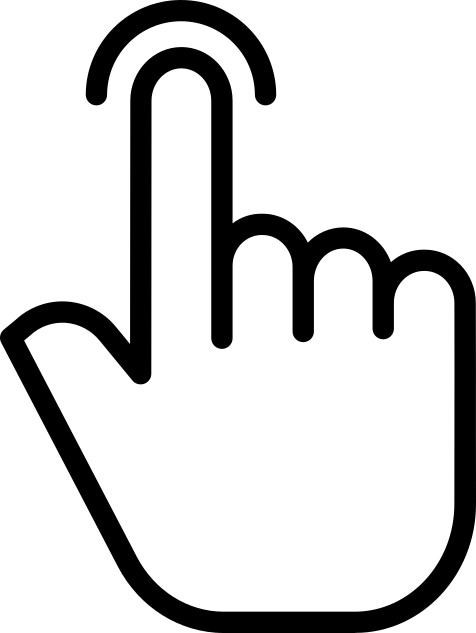
\includegraphics[width=0.05\textwidth]{static/dedo.png}};
    \node[const, above=of d] (nd) {\Large $s$} ;

    \edge {r} {d};
    }
  \caption{Las pistas dependen de dónde está el regalo.}
  \label{fig:modelo_causal_base}
\end{figure}

Ahora nuestra distribución de creencias no es sobre una variable, como hicimos antes, es sobre las dos variables.
\begin{equation}
 \text{Creencia}(r_i, s_j)
\end{equation}
Esto se lee como ``la creencia de que ocurran ambos: que el regalo esté en la cada $i$, $r_i$, y que la persona señale la caja $j$, $s_j$''.
%
Para determinar la creencia honesta en casos donde hay varias variables vinculadas por un modelo causal, sigue siendo necesario dividir la creencia en partes iguales, pero ahora por los caminos del modelo causal.

\begin{figure}[ht!]     
 \centering
    \tikz{
    \node[latent, draw=white, yshift=0.6cm] (b0) {$ 1$};

    \node[latent,below=of b0,yshift=0.6cm, xshift=-3cm] (r1) {$r_1$};
    \node[latent,below=of b0,yshift=0.6cm] (r2) {$r_2$};
    \node[latent,below=of b0,yshift=0.6cm, xshift=3cm] (r3) {$r_3$};

    \node[latent, below=of r1, draw=white, yshift=0.6cm] (br1) {$\frac{1}{3}$};
    \node[latent, below=of r2, draw=white, yshift=0.6cm] (br2) {$\frac{1}{3}$};
    \node[latent, below=of r3, draw=white, yshift=0.6cm] (br3) {$\frac{1}{3}$};

    \node[latent,below=of br1,yshift=0.6cm, xshift=-0.7cm] (r1d2) {$s_2$};
    \node[latent,below=of br1,yshift=0.6cm, xshift=0.7cm] (r1d3) {$s_3$};

    \node[latent,below=of r1d2,yshift=0.6cm,draw=white] (br1d2) {$\frac{1}{3}\frac{1}{2}$};
    \node[latent,below=of r1d3,yshift=0.6cm, draw=white] (br1d3) {$\frac{1}{3}\frac{1}{2}$};

    \node[latent,below=of br2,yshift=0.6cm, xshift=-0.7cm] (r2d1) {$s_1$};
    \node[latent,below=of br2,yshift=0.6cm, xshift=0.7cm] (r2d3) {$s_3$};
    \node[latent,below=of br3,yshift=0.6cm, xshift=-0.7cm] (r3d1) {$s_1$};
    \node[latent,below=of br3,yshift=0.6cm, xshift=0.7cm] (r3d2) {$s_2$};

    \node[latent,below=of r2d1,yshift=0.6cm, draw=white] (br2d1) {$\frac{1}{3}\frac{1}{2}$};
    \node[latent,below=of r2d3,yshift=0.6cm,draw=white] (br2d3) {$\frac{1}{3}\frac{1}{2}$};
    \node[latent,below=of r3d1,yshift=0.6cm, draw=white] (br3d1) {$\frac{1}{3}\frac{1}{2}$};
    \node[latent,below=of r3d2,yshift=0.6cm,draw=white] (br3d2) {$\frac{1}{3}\frac{1}{2}$};

    \edge[-] {b0} {r1,r2,r3};
    \edge[-] {r1} {br1};
    \edge[-] {r2} {br2};
    \edge[-] {r3} {br3};
    \edge[-] {br1} {r1d2,r1d3};
    \edge[-] {r1d2} {br1d2};
    \edge[-] {r1d3} {br1d3};
    \edge[-] {br2} {r2d1, r2d3};
    \edge[-] {br3} {r3d1,r3d2};
    \edge[-] {r2d1} {br2d1};
    \edge[-] {r2d3} {br2d3};
    \edge[-] {r3d1} {br3d1};
    \edge[-] {r3d2} {br3d2};
    }
  \caption{Dividir las creencias en partes iguales por los caminos del modelo causal}
  \label{fig:dividir_creencias_modelo_causal}
\end{figure}

Esto nos determina la distribución de creencias conjunta honesta.
Decimos conjunta porque estamos hablando de creencias sobre más de una variable a la vez.
La tabla \ref{tab:creencia_conjunta_honesta} la completamos con las creencias que tienen los caminos en la figura \ref{fig:dividir_creencias_modelo_causal}.
\begin{table}[H]
  \centering
  Creencia$(r,s)$ \\ \vspace{0.3cm}
 \begin{tabular}{c|c|c|c|} \setlength\tabcolsep{0.4cm} 
        & \, $r_1$ \, &  \, $r_2$ \, & \, $r_3$ \, \\ \hline 
  $s_1$  & $0$ & $1/6$ & $1/6$  \\ \hline
  $s_2$  & $1/6$ & $0$ & $1/6$   \\ \hline
       $s_3$ & $1/6$ & $1/6$ & $0$   \\ \hline 
\end{tabular}
\caption{Distribución de creencias conjunta honesta}
\label{tab:creencia_conjunta_honesta}
\end{table}

Conseguimos la distribución de creencias de que ocurran ambas cosas a la vez.
¿Cuál es la creencia de que el regalo esté en las cajas?
\begin{equation}
 \text{Creencia}(r_i)
\end{equation}

\todo[inline, color=gray!50]{Explicar esto primero de forma intuitiva. Vas a estar introduciendo la regla de la suma.}

Finalmente, en la tabla \ref{tab:creencia_marginal_honesta} mostramos el resultado de integrar las creencias conjunta para obtener la creencia de una única variable.
\begin{table}[H]
  \centering
    Creencia$(r,s)$ \\ \vspace{0.3cm}
    \begin{tabular}{c|c|c|c||c} \setlength\tabcolsep{0.4cm} 
            & \, $r_1$ \, &  \, $r_2$ \, & \, $r_3$ \, & \phantom{\bm{$1/3$}} \\ \hline 
    $s_1$ & $0$ & $1/6$ & $1/6$ & $1/3$ \\ \hline
    $s_2$ & $1/6$ & $0$ & $1/6$ & $1/3$ \\ \hline
    $s_3$ & $1/6$ & $1/6$ & $0$ & $1/3$ \\ \hline \hline
            & $1/3$ & $1/3$ & $1/3$ & $1$ \\ 
    \end{tabular}
  \caption{Integrar creencias.}
  \label{tab:creencia_marginal_honesta}
\end{table}

\begin{framed} \centering
Regla 1 \\
\textbf{Integrar las creencias en partes iguales}
\end{framed}

En términos formales esto no es más que sumar todos los términos de la conjunta.
\begin{equation*}
\text{Creencia}(r_i) = \sum_j \text{Creencia}(r_i, s_j) 
\end{equation*}

\todo[inline, color=gray!50]{expicar esta función, cómo se lee la sumatoria, que signific el subíndice de la sumatoria, etc}

Ya sabemos como definir distribución de creencias honestas cuando no tenemos información.
Ahora, ¿cómo se actualizan las distribución de creencia de forma honesta luego de obtener información nueva?
Por ejemplo, si no ponemos en duda que la pista del que nos dan depende de las relación causal expuesta en la figura \ref{fig:modelo_causal_base}, ¿cuál es la forma honesta de actualizar creencias?

\begin{figure}[H]
\centering
 \tikz{ %
        
         \node[factor, minimum size=1cm] (p1) {} ;
         \node[det, minimum size=1cm, xshift=1.5cm] (p2) {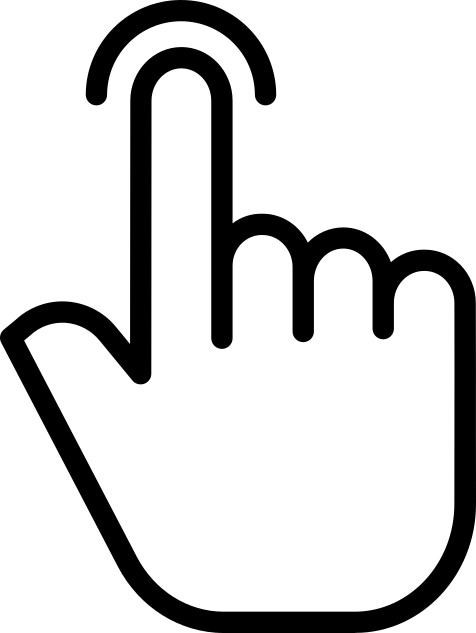
\includegraphics[width=0.03\textwidth]{static/dedo.png}} ;
         \node[factor, minimum size=1cm, xshift=3cm] (p3) {} ;

         \node[const, above=of p1, yshift=.15cm] (fp1) {$?$};
         \node[const, above=of p2, yshift=.15cm] (fp2) {$0$};
         \node[const, above=of p3, yshift=.15cm] (fp3) {$?$};
         \node[const, below=of p2, yshift=-.10cm, xshift=0.3cm] (dedo) {};
        } 
 \caption{Recibimos una pista que nos dice dónde no está el regalo.}
 \label{fig:pista_no_regalo}
\end{figure}

Si ya tenemos una creencia honesta previa, y ahora vemos un dato, lo que podemos hacer es quedarnos con la creencia previa que es compatible con el dato.
El resto fue creencia que asignamos opciones que ya no son compatibles con la realidad, el dato. 

\begin{table}[H]
\centering
Creencia$(r,s_2)$ \\ \vspace{0.3cm}
 \begin{tabular}{c|c|c|c||c} \setlength\tabcolsep{0.4cm} 
        & \, $r_1$ \, &  \, $r_2$ \, & \, $r_3$ \, &  \phantom{\bm{$1/3$}} \\ \hline 
  &  &  &  & \\ \hline
  $s_2$ & $1/6$ & $0$ & $1/6$ & $1/3$\\ \hline
  &  &  & &  \\ 
\end{tabular}
\caption{Creencias conjunta honestas compatible con el dato}
\label{tab:creencia_condicional_proporcional}
\end{table}

De la creencia conjunta honesta, solo sobrevive aquella que es compatible con el dato, que la pista fue la puerta 2.
 
\vspace{0.3cm}

Después de haber visto los datos, la creencia total se redujo a $1/3$.
Pero si esta es ahora nuestra creencia total, quisieramos volver a expresarla como $1$, en el sentido de que representa el $100$\% de nuestras creencias actuales.
Esto se logra normalizando, dividiendo por la creencia total que nos quedó $1/3$.
\begin{table}[H]
\centering
Creencia$(r|s_2)$ \\ \vspace{0.3cm}
 \begin{tabular}{c|c|c|c||c} \setlength\tabcolsep{0.4cm} 
        & \, $r_1$ \, &  \, $r_2$ \, & \, $r_3$ \, &  \phantom{\bm{$1/3$}} \\ \hline 
  &  &  &  & \\ \hline
  $s_2$ & $1/2$ & $0$ & $1/2$ & $1$ \\ \hline
  &  &  & &  \\ 
\end{tabular}
\caption{Creencia condicional}
\label{tab:creencia_condicional}
\end{table}

Es decir, a partir de la creencia honesta inicial y la pista podemos decir que la creencia honesta actualizada en este caso es
\begin{figure}[H]
 \centering
\tikz{ %
        
         \node[factor, minimum size=1cm] (p1) {} ;
         \node[det, minimum size=1cm, xshift=1.5cm] (p2) {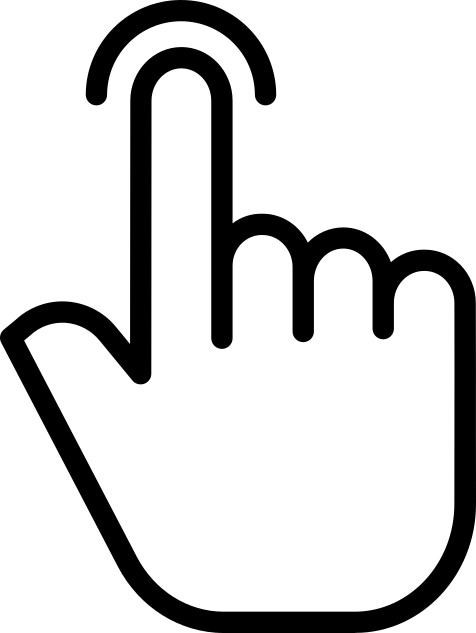
\includegraphics[width=0.03\textwidth]{static/dedo.png}} ;
         \node[factor, minimum size=1cm, xshift=3cm] (p3) {} ;

         \node[const, above=of p1, yshift=.15cm] (fp1) {$1/2$};
         \node[const, above=of p2, yshift=.15cm] (fp2) {$0$};
         \node[const, above=of p3, yshift=.15cm] (fp3) {$1/2$};
         \node[const, below=of p2, yshift=-.10cm, xshift=0.3cm] (dedo) {};
        
        } 
\caption{Creencia actualizada.}
\label{fig:creencia_condicional}
\end{figure}

\begin{framed} \centering
  Regla 2 \\
\textbf{Contextualizar las creencias en partes iguales} 
\end{framed}

\begin{align*}
 P(r|s_2) = \frac{P(r, s_2)}{P(s_2)}
 \end{align*} 
 
 \todo[inline, color=gray!50]{Explicar esta función.}


\section{Las reglas de la probabilidad}

\begin{equation*}
  \text{Marginal}_{i} = \sum_j \text{Conjunta}_{ij}  \ \ \ \ \ \ \ \ \  \ \ \ \ \ \ \ \ \ \ \ \ \ \ \  \text{Condicional}_{j|i} = \frac{\text{Conjunta}_{ij}}{\text{Marginal}_{i}}
\end{equation*}

\todo[inline, color=gray!50]{Volver a hablar de las regla 1 (integrar creencias) y de la regla 2 (contextualizar creencias).}

\begin{equation}\tag{\text{Regla de la suma}}
 P(r) = \sum_j P(r,s_j)
\end{equation}
Cualquier distribución marginal puede ser obtenida integrando la distribución conjunta

\begin{equation}\tag{\text{Regla del producto}}
 P(r,s) = P(s|r)P(r)
\end{equation}
Cualquier distribución conjunta puede ser expresada como el producto de distribuciones condicionales uni-dimensionles.

\vspace{0.3cm}

El teorema de Cox \cite{citarbiblio} dice que estas reglas que las encontramos intuitivamente son las únicas reglas que grantizan:
\begin{itemize} \setlength\itemsep{0cm}
 \item[$\bullet$] Representar las creencias con valores reales 
 \item[$\bullet$] Actualizar las creencias en la direcci\'on de la evidencia
 \item[$\bullet$] Consistencia, todos los caminos conducen a la misma conslusión
 \end{itemize}
 
Es decir, estas reglas no son reglas arbitrarias.
Son las reglas óptimas en el sentido de la honestidad, utilizan toda la información disponible, ni más ni menos, por lo que son de validez intercultural.

\vspace{0.3cm}

\todo[inline, color=gray!50]{Escribir mejor la conlusión interculutral, las consecuencias de que sean reglas honestas y teóricamente las únicas posibles}

In 1946, thanks to Cox, it was now a theorem that any set of rules for conducting inference, in which we represent degrees of plausibility by real numbers, is necessarily either equivalent to the Laplace-Jefreys rules, or inconsistent
 
\section{Monty Hall}

\todo[inline, color=gray!50]{Explicar monty hall}

\begin{figure}[H]
\centering
\tikz{        
    
    \node[latent] (d) {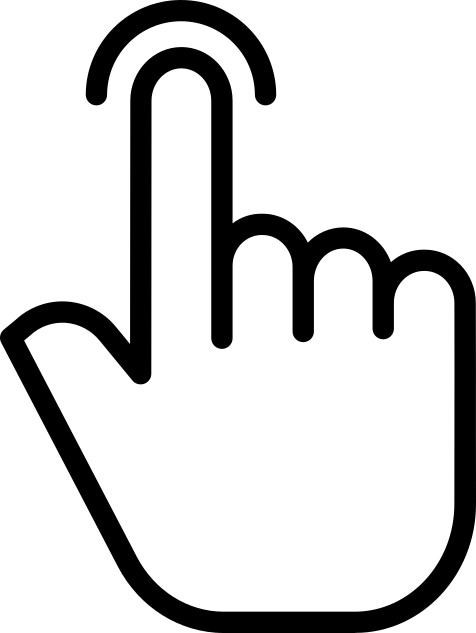
\includegraphics[width=0.05\textwidth]{static/dedo.png}} ;
    \node[const,above=of d] (nd) {\Large $s$} ;
    
    \node[latent, above=of d, xshift=-1.5cm] (r) {
\includegraphics[width=0.06\textwidth]{static/regalo.png}} ;
    \node[const,above=of r] (nr) {\Large $r$} ;
    
    \node[latent, fill=black!30, above=of d, xshift=1.5cm] (c) {
\includegraphics[width=0.06\textwidth]{static/cerradura.png}} ;
    \node[const,above=of c] (nc) {\Large $c$} ;
    
    \edge {r,c} {d};
}
\caption{Monty Hall}
\label{fig:modelo_monty_hall}
\end{figure}

Escribir ...


\begin{figure}[H]
\centering
\tikz{ %
         \node[factor, minimum size=1cm] (p1) {} ;
         \node[factor, minimum size=1cm, xshift=1.5cm] (p2) {} ;
         \node[factor, minimum size=1cm, xshift=3cm] (p3) {} ;

         \node[const, above=of p1, yshift=.15cm] (fp1) {$1/3$};
         \node[const, above=of p2, yshift=.15cm] (fp2) {$1/3$};
         \node[const, above=of p3, yshift=.15cm] (fp3) {$1/3$};
        
        } 
\caption{Escribir ...}
\label{fig:monty_hall_regalo}
\end{figure}

Escribir ...

\begin{figure}[H]
\centering
\tikz{ %
         \node[factor, minimum size=1cm] (p1) {
\includegraphics[width=0.025\textwidth]{static/cerradura.png}} ;
         \node[factor, minimum size=1cm, xshift=1.5cm] (p2) {} ;
         \node[factor, minimum size=1cm, xshift=3cm] (p3) {} ;

         \node[const, above=of p1, yshift=.15cm] (fp1) {$1/3$};
         \node[const, above=of p2, yshift=.15cm] (fp2) {$1/3$};
         \node[const, above=of p3, yshift=.15cm] (fp3) {$1/3$};
        
        } 
\caption{Escribir ...}
\label{fig:monty_hall_cerradura}
\end{figure}

Escribir ...

\begin{figure}[H]
 \centering
\tikz{ %
        
         \node[factor, minimum size=1cm] (p1) {
\includegraphics[width=0.025\textwidth]{static/cerradura.png}} ;
         \node[det, minimum size=1cm, xshift=1.5cm] (p2) {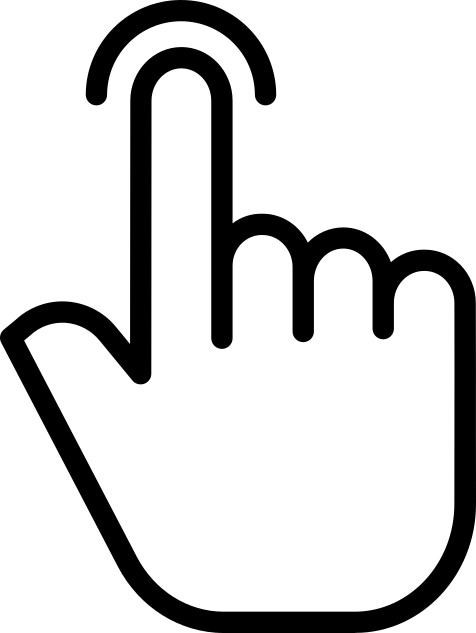
\includegraphics[width=0.03\textwidth]{static/dedo.png}} ;
         \node[factor, minimum size=1cm, xshift=3cm] (p3) {} ;
         
         \node[const, above=of p1, yshift=.15cm] (fp1) {$?$};
         \node[const, above=of p2, yshift=.15cm] (fp2) {$0$};
         \node[const, above=of p3, yshift=.15cm] (fp3) {$?$};
         \node[const, below=of p2, yshift=-.10cm, xshift=0.3cm] (dedo) {};
        
        } 
\caption{Escribir ...}
\label{fig:monty_hall_pista}
\end{figure}

Escribir ...


\begin{figure}[H]
\centering
\tikz{
\node[latent, draw=white, yshift=0.8cm] (b0) {$1$};
\node[latent,below=of b0,yshift=0.8cm, xshift=-2cm] (r1) {$r_1$};
\node[latent,below=of b0,yshift=0.8cm] (r2) {$r_2$};
\node[latent,below=of b0,yshift=0.8cm, xshift=2cm] (r3) {$r_3$};

\node[latent, below=of r1, draw=white, yshift=0.8cm] (br1) {$\frac{1}{3}$};
\node[latent, below=of r2, draw=white, yshift=0.8cm] (br2) {$\frac{1}{3}$};
\node[latent, below=of r3, draw=white, yshift=0.8cm] (br3) {$\frac{1}{3}$};

\node[latent,below=of br1,yshift=0.8cm] (c11) {$c_1$};
\node[latent,below=of br2,yshift=0.8cm] (c12) {$c_1$};
\node[latent,below=of br3,yshift=0.8cm] (c13) {$c_1$};

\node[latent, below=of c11, draw=white, yshift=0.8cm] (bc11) {$\frac{1}{3}$};
\node[latent, below=of c12, draw=white, yshift=0.8cm] (bc12) {$\frac{1}{3}$};
\node[latent, below=of c13, draw=white, yshift=0.8cm] (bc13) {$\frac{1}{3}$};

\node[latent,below=of bc11,yshift=0.8cm, xshift=-0.7cm] (r1d2) {$s_2$};
\node[latent,below=of bc11,yshift=0.8cm, xshift=0.7cm] (r1d3) {$s_3$};
\node[latent,below=of bc12,yshift=0.8cm] (r2d3) {$s_3$};
\node[latent,below=of bc13,yshift=0.8cm] (r3d2) {$s_2$};

\node[latent,below=of r1d2,yshift=0.8cm,draw=white] (br1d2) {$\frac{1}{3}\frac{1}{2}$};
\node[latent,below=of r1d3,yshift=0.8cm, draw=white] (br1d3) {$\frac{1}{3}\frac{1}{2}$};
\node[latent,below=of r2d3,yshift=0.8cm,draw=white] (br2d3) {$\frac{1}{3}$};
\node[latent,below=of r3d2,yshift=0.8cm,draw=white] (br3d2) {$\frac{1}{3}$};

\edge[-] {b0} {r1,r2,r3};
\edge[-] {r1} {br1};
\edge[-] {r2} {br2};
\edge[-] {r3} {br3};
\edge[-] {br1} {c11};
\edge[-] {br2} {c12};
\edge[-] {br3} {c13};
\edge[-] {c11} {bc11};
\edge[-] {c12} {bc12};
\edge[-] {c13} {bc13};
\edge[-] {bc11} {r1d2,r1d3};
\edge[-] {bc12} {r2d3};
\edge[-] {bc13} {r3d2};
\edge[-] {r1d2} {br1d2};
\edge[-] {r1d3} {br1d3};
\edge[-] {r2d3} {br2d3};
\edge[-] {r3d2} {br3d2};
}
\caption{}
\label{fig:monty_hall_caminos}
\end{figure}

Escribir ...

\begin{table}[H]
\centering
$P(r,s)$ \\ \vspace{0.3cm}
 \begin{tabular}{c|c|c|c|} \setlength\tabcolsep{0.4cm} 
        & \, $r_1$ \, &  \, $r_2$ \, & \, $r_3$ \, \\ \hline 
  { $s_2$}  & {$1/6$} & {$0$} & {$1/3$} \\ \hline
       {$s_3$} & {$1/6$} & {$1/3$} & {$0$}  \\ \hline
    \end{tabular}
\caption{Escribir ...}
\label{tab:monty_hall_conjunta}
\end{table}

Escribir ...

\begin{table}[H]
\centering
$P(r,s)$ \\ \vspace{0.3cm}
 \begin{tabular}{c|c|c|c||c} \setlength\tabcolsep{0.4cm} 
        & \, $r_1$ \, &  \, $r_2$ \, & \, $r_3$ \, & \\ \hline 
  { $s_2$}  & {$1/6$} & {$0$} & {$1/3$} & {$1/2$} \\ \hline
       {$s_3$} & {$1/6$} & {$1/3$} & {$0$} & {$1/2$} \\ \hline
              & {$1/3$} & {$1/3$} & {$1/3$}  & {$1$} \\ 
\end{tabular}
\caption{Escribir ...}
\label{tab:monty_hall_conjunta_y_marginal}
\end{table}

Escribir ...

\begin{table}[H]
 \centering
$P(r,s_2)$ \\ \vspace{0.3cm}
 \begin{tabular}{c|c|c|c||c} \setlength\tabcolsep{0.4cm} 
        & \, $r_1$ \, &  \, $r_2$ \, & \, $r_3$ \, & \\ \hline 
        { $s_2$}  & {$1/6$} & {$0$} & {$1/3$} & {$1/2$} \\ \hline
\end{tabular}
\caption{}
\label{tab:monty_hall_conjunta_compatible}
\end{table}

Escribir ...

\begin{table}[H]
 \centering
$P(r|s_2)$ \\ \vspace{0.3cm}
 \begin{tabular}{c|c|c|c||c} \setlength\tabcolsep{0.4cm} 
        & \, $r_1$ \, &  \, $r_2$ \, & \, $r_3$ \, & \phantom{$1/2$}\\ \hline 
  { $s_2$}  & {$1/3$} & {$0$} & {$2/3$} & {$1$} \\ \hline
\end{tabular}
\caption{}
\label{tab:monty_hall_condicional}
\end{table}

Escribir ...

\begin{figure}[H]
 \centering
\tikz{ %
        
         \node[factor, minimum size=1cm] (p1) {
\includegraphics[width=0.025\textwidth]{static/cerradura.png}} ;
         \node[det, minimum size=1cm, xshift=1.5cm] (p2) {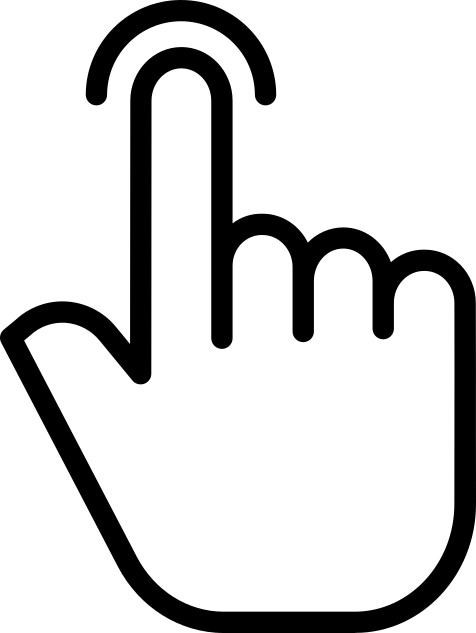
\includegraphics[width=0.03\textwidth]{static/dedo.png}} ;
         \node[factor, minimum size=1cm, xshift=3cm] (p3) {} ;
         
         \node[const, above=of p1, yshift=.15cm] (fp1) {$1/3$};
         \node[const, above=of p2, yshift=.15cm] (fp2) {$0$};
         \node[const, above=of p3, yshift=.15cm] (fp3) {$2/3$};
         \node[const, below=of p2, yshift=-.10cm, xshift=0.3cm] (dedo) {};        } 
\caption{Escribir}
\label{fig:monty_hall_condicional}
\end{figure}

Escribir ...




\newpage

\section{Base empírica}

\section{Selección de modelos}

\section{Conclusiones}


\chapter{Modelos de estimación de habilidad (TTT)}

\chapter{Sistema de estimación para el juego Go (AAGo).}

\chapter{Efecto de los equipos sobre el aprendizaje (faithfull-sinergia)}

\chapter{Efecto de la topología sobre el aprendizaje.}


\end{document}
